\documentclass[11pt]{report}

\usepackage{graphicx}
\usepackage{hyperref}
\usepackage{url}
\usepackage{epstopdf}
\usepackage{listings}
\usepackage{color}
\usepackage{ulem}

\renewcommand\bibname{References}

% reference commands
\newcommand{\fig}[1]{Figure ~\ref{fig:#1}}
\newcommand{\tab}[1]{Figure ~\ref{tab:#1}}
\newcommand{\sect}[1]{Section ~\ref{sec:#1}}

\setcounter{secnumdepth}{3}
\setcounter{tocdepth}{3}
\parindent 0pt
\parskip 8pt

%Gummi|061|=)
\title{Project CS 2012 Product Report\\Uppsala University\\}

\author{Daniele Bacarella\\
		Jon Borglund\\
		Paolo Boschini\\
		Kiril Goguev\\
		Faroogh Hassan\\
		Marcus Ihlar\\
		Alexander Lindholm\\
		Knut Lorenzen\\
		Harold Mart\'{i}nez\\
		Thomas Nordstr\"om\\
		Thiago Costa Porto\\
		Linus Sunde\\
		Kim-Anh Tran
}

\date{}
\begin{document}

\maketitle

\begin{abstract}
In Information Centric Networking (ICN), content is delivered to users based on
the name of the requested resource without taking into consideration its physical location.
Based on the NetInf protocol, an Android application backed by an Erlang implementation of a
Name Resolution Service was implemented and both products are presented in this report.
By communicating with each other, the systems store, share and retrieve data objects in an ICN fashion.
In situations of network congestion content is difficult or impossible to retrieve.
Using ICN, the system can provide alternate transfer methods to facilitate the delivering of content.
\end{abstract}

\section{Glossary}
\textbf{API} - Application Programming Interface\\
\textbf{CH} - Content Handler\\
\textbf{CL} - Convergence Layer\\
\textbf{ERNI} - Erlang NetInf\\
\textbf{EH} - Event Handler\\
\textbf{HTML} - HyperText Markup Language\\
\textbf{HTTP} - HyperText Transfer Protocol\\
\textbf{ICN} - Information-centric Networking\\
\textbf{IO} - Information Object\\
\textbf{IDE} - Integrated Development Environment\\
\textbf{JSON} - JavaScript Object Notation\\
\textbf{LRS} - Local Resolution Service\\
\textbf{MAC} - Media Access Control\\
\textbf{MH} - Message Handler\\
\textbf{NDO} - Named Data Object\\
\textbf{NRS} - Name Resolution Service\\
\textbf{NetInf} - Network of Information\\
\textbf{OTP} - Open Telecom Platform\\
\textbf{SAIL} - Scalable and Adaptive Internet soLutions\\
\textbf{SDK} - Software Development Kit\\ 
\textbf{SQL} - Structured Query Language\\
\textbf{TCP/IP} - Transmission Control Protocol/Internet Protocol\\ 
\textbf{UDP} - User Datagram Protocol\\
\textbf{URL} - Uniform Resource Locator\\
\textbf{URI} - Uniform Resource Identifier\\









\tableofcontents

\chapter{Introduction}

Nowadays the usage of technical devices has become irreplaceable. But with increasing
densification of devices comes network congestion: problems of
browsing the web during a train ride or a concert are apparent. Simply put, the current
location-based networking was not addressed for today's idea of massive content sharing. 
In order to face these problems Information-Centric Networking (ICN) was introduced. For
more information about ICN and all its existing architectures (Data-Oriented Network Architecture (DONA),
Content-Centric Networking (CCN), Publish-Subscribe Internet Routing Paradigm (PSIRP) and Network of Information (NetInf)) 
see \cite{netinf}.
The idea behind ICN is to shift the focus from hosts that serve a content to the actual objects that
are shared. More specifically, these Named Data Objects (NDO) shall no longer be coupled
to a host that is owning the content, but shall ideally be retrievable from \textit{anywhere}.

This report picks a proof-of-concept implementation of the usage of NetInf
(see \sect{netinf}), one out of four concepts that realize ICN. The software was
developed in the context of the 
\textit{Project Computer Science}\footnote{\url{http://www.it.uu.se/edu/course/homepage/projektDV/ht12}},
a course under the supervision of Olle G\"{a}llmo and in cooperation with Ericsson Research \cite{ericsson}
in 2012/2013. The goals set for this project are listed in \sect{goals}. 

The product itself consists of two separate parts developed by two development teams within the same project group. One is an Erlang \cite{erlang} implementation of a Name Resolution Service (NRS) with streaming capabilities.
The other product is a browser application called "Elephant" for Android \cite{android}  phones that takes advantage of NetInf services that
are based on OpenNetInf \cite{opennetinf}, an open source Java implementation of NetInf. 

Both products are described more in detail in \sect{product}. For a thorough understanding
of the implementation and extension of the current state, preliminaries and system architecture decisions are 
described in \sect{preliminaries} and \sect{architecture}. 
The performance of both products are evaluated in \sect{evaluation} and based on the results,
\sect{conclusions} discusses the future work and draws conclusions for the developed products. Finally, the appendix contains installation as well as maintenance instructions.


\chapter{Preliminaries}
\label{sec:preliminaries}
\subsection{Information-centric Networking}
\label{sec:netinf}
The Internet was originally designed based on a host-centric paradigm (one-to-one communication), where users explicitly connect to hosts in order to use services and retrieve resources. In the early days this worked well due to the low amount of users per host, but as the internet gained popularity the use of services began to increase. Over the past decades, the host-centric approach has become a growing impediment for services with large user bases, with workarounds like load-balancing and content delivery networks to circumvent bandwidth bottle necks in place. Today most traffic involves transferring of audio/video media and social networking content, both relying on one-to-many communication. Information centric networking (ICN) is a research field aiming to redesign the internet in a fundamental way for today's and the near future usage patterns. In ICN, the actual host providing a specific resource or service can be arbitrary and therefore unknown to the user. Instead of connecting to a host, the user queries the network as a whole. This enables low-level caching in every network node, so that repeated forwarding of identical information can be minimised and bandwidth be used more efficiently. The main challenges in ICN are the ways of addressing information units and integration with existing, host-centric networks. At this time ICN only exists in the form of independent research projects (e.g. NetInf), with no cross-industry standards on the horizon yet \cite{ICNarticle}. 


\subsection{Network of Information}
Network of Information(NetInf) is one of the first approaches proposed by the 4WARD project. \cite{4ward} This ICN paradigm was intended to deal with the issues that the current Host-Centric Networks suffer from. Every object on the network is called a Named Data Object(NDO) and is self-verifying. This leads to the user being able to request a certain object, an NDO, and fetch it from any source without worrying who or where it gets it from. The NDO can verify itself by using its own hash value as part of its name along with the used hash-algorithm.
A lot has changed in NetInf since the 4WARD project made the first draft. Currently the most recent versions are managed by the SAIL project. \cite{netinfproto}

\subsection{OpenNetInf}
OpenNetInf \cite{opennetinf} is an open source Java implementation of NetInf developed at the University of Paderborn. OpenNetInf is still in the very early development phase and mainly aimed at research. The frontend development team decided to use OpenNetInf as the starting point for the android client's NetInf functionality, but still had to implement and extend it to provide the needed functionality. One reason for choosing OpenNetInf, rather than starting from scratch, was not having to reinvent the wheel. It was also a chance to contribute to an existing project. Another reason was the closely related work done in a previous master thesis \cite{masterthesis} which used OpenNetInf.

\section{Development Languages}
\subsection{Java-Android}

Elephant was developed for Android, an operating system targeted at mobile devices. This made it all but natural to use Java since this is the primary supported language for Android applications. The fact that both OpenNetInf and a closely related previous master thesis \cite{hugomiguel} also used Java further solidified this decision. Java is an imperative object-orient programming language. Access to Android API libraries and other tools needed for development are provided by the Android SDK.

\subsection{Erlang}
Erlang is a concurrent, functional, fault-tolerant language with great scalability and ease of distribution. It was developed by Ericsson in the mid 80's and became open source 1998.\cite{otpInAction} These factors among others such as the client being Ericsson Research made Erlang the choice of language for the NRS implementation.
Another reason for choosing Erlang is that it uses the idea of modules and nodes as a primary platform for serving a function, which allowed the product to be broken up into several parts which could be developed concurrently.
\subsection{Javascript}
Javascript was used when the backend group decided to create a simple http interface to the NetInf Name Resolution server in order to show a proof of concept (NetInf streaming). Javascript was used to calculate the hash of files for streaming as well as for asynchronious communication with the NRS.

\chapter{Goals and Scope}
\label{sec:goals}
\section{Frontend}

\subsection{NetInf Enabled Browser}

The goal of the frontend is to produce a NetInf enabled browser for Android devices. The browser utilizes NetInf technology to retrieve web pages from other nearby devices and/or caching nodes in order to reduce the usage of shared 3G uplinks. The NetInf messages should conform to the NetInf HTTP convergence layer \cite{netinfproto}. Web pages are split into several parts to be able to benefit from being available from multiple sources.

NetInf protocol mandates the browser have the possibility to:

\begin{itemize}
	\item Inject existing web pages into the NetInf network as NDOs.
	\item Given a traditional web URL be able to find the corresponding NDO.
	\item Get NDOs from other devices.
\end{itemize}

The following problems are considered to be out of scope:

\begin{itemize}
	\item Privacy
	\item Security
	\item Dynamic Content
	\item Battery Consumption
	\item Bluetooth Congestion
\end{itemize}

Privacy and security are both very important aspects, but would require complex considerations. They are areas that require future work.

Dynamic content is relevant since a lot of content that is of interest to many users is dynamic and changes often (e.g. newspapers, Facebook, Twitter). However this adds a lot of complexity to the problem since dynamic content means the mappings from traditional web URLs to NDOs are constantly changing.

Battery consumption is a serious issue in this type of application. The application uses Bluetooth which is a battery draining technology. The simplest solution here is to let the user disable Bluetooth. Hopefully the problem of heavy battery consumption will be solved by future technological advancements.

A final problem that is not taken into consideration is possible congestion in the Bluetooth network due to a large amount of devices running simultaneously.
\section{Backend}
This section describes the goals and scope set by the backend team for this product.

\subsection{Goals}
The following goals were set for the Erlang implementation of the Name Resolution Service (NRS):
\begin{enumerate}
 \item {Build an NRS for the Erlang NetInf application.}\\
 \item {Be able to publish, store and retrieve Named Data Objects (NDO's) in a NetInf network.}\\
 \item {Make each NetInf node a caching node that can store NDO's.}\\
 \item {Make the back-end processes distributed, concurrent and fault tolerant.}\\ 
 \item {Be able to stream video using our Erlang NetInf application.}\\
  \end{enumerate}

\subsection{Scope}
The scope of the NRS application is limited to providing all the functionalities outlined in the NetInf Protocol draft document. \cite{netinfproto} This document outlines what information a NetInf Get, Publish and Search message should contain. It also defines how a Get, Publish and Search response message should look like. Apart from that it also covers specifications for the HTTP and UDP convergence layers. We made sure that our application followed all these specifications accurately. Providing video streaming was not part of the scope at the beginning of this project but at the client's request preliminary(proof-of-concept) work was done, however readers should note that the video streaming is not meant to be a complete product and the development team encourages further research into this product.


\chapter{Product Description}
\label{sec:product}

\section {Frontend - Android Client}

\section {Backend}

The customer agreed on having an Erlang NetInf NRS. The backend product implements the, as of writing, current draft of the NetInf Protocol\cite{netinfproto} in a purely functional language. The product promises a high level of scalability and fault-tolerance. The client initially asked for only the NRS as a product however the backend team was able to complete the initial product in a timely manner, allowing for applications of this network technology to be explored. 


\subsection {Erlang NetInf Name Resolution Service}
The first of the two deliverables from the backend team to the customer. The Erlang NetInf NRS provides a new way to organize and retrieve data on the Internet. Based on an initial NetInf NRS protocol draft from development teams such as SAIL and Ericsson Research\cite{netinfproto}. This product allows for flexibility and extension of the existing protocol.

Erlang's concept of modularization allowed the team to break up the NRS functionality into distinctive convergence layers, runtime database switching, and even allow for a proof-of-concept data streaming client/protocol. 

\subsection{NetInf Video Streaming Client/Protocol}

The last of the deliverables from the backend team. The customer requested a proof-of-concept video streaming protocol and HTML client interface which lies on top of the Erlang NetInf NRS technology. The streaming protocol is a completely new addition to the NetInf draft\cite{netinfproto}. The team developed a way to utilize the code and transporting mechanism of the first product in order to stream video content. Along with the protocol outlined in Appendix C \ref{VideoDraft}, the team has created a HTTP interface client which allows the user to see the streaming protocol in action in addition to accessing the NRS functionality. This particular product was not specified in the initial conversations with the customer in September, but was added late in the development cycle and is a proof-of-concept.

\subsubsection{First Implementation}
In addition to normal NRS functionality, a HTTP transfer-dispatcher had to be implemented in order to transfer of chunks between clients. The streaming works by clients subscribing to a stream from a specific NRS. Once connected the stream the client with a constant interval will ask the NRS where to find these chunks. All the chunks are transferred via the transfer-dispatcher.
The playback of the video chunks is done by polling the local NRS, this implies that every client has its own NetInf node running. See figure \ref{fig:stream-seqorgmod}. The benefit of using this approach is that only one NDO containing the filename has to be published. The receiver can then derive the chunks locations, by appending the chunk number to the end of the locators provided in the filename NDO.

\begin{figure}[h!]
	\centering
		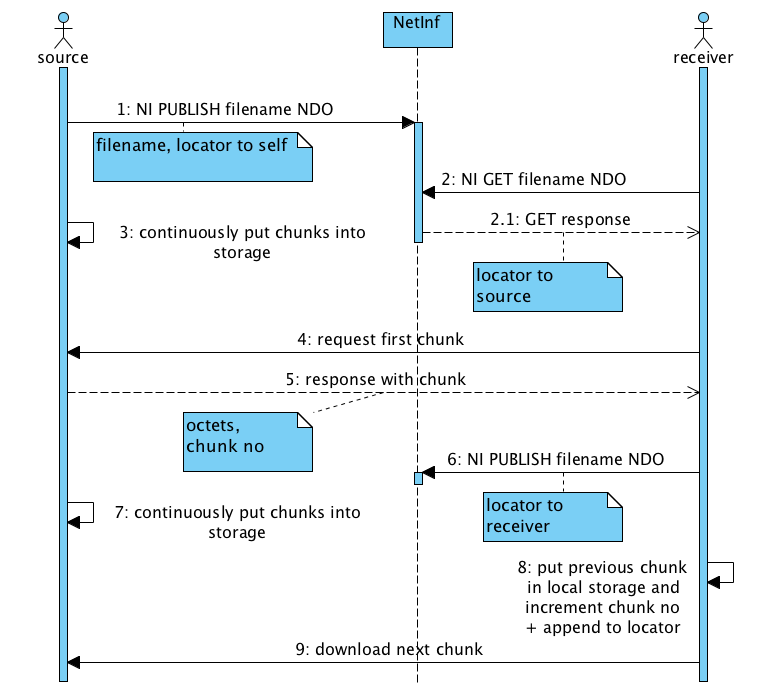
\includegraphics[width=0.75\textwidth]{./img/sequence_diagram_streaming_orgmod.png}
    	\caption{Original/Modified Chunked Data Transfer}
	\label{fig:stream-seqorgmod}
\end{figure}

\subsubsection{Modified NetInf Streaming}
Due to a request from the customer a more true NetInf implementation of streaming was implemented. Instead of using the transfer-dispatcher between the client nodes a workaround was added that disabled content validation, this resulted in fetching of chunks via NetInf messages. The polling logic is still the same as first implementation, seen in figure \ref{fig:stream-seqorgmod}. Instead of using ordinary HTTP locators, the receiver is required to modify the \textit{NetInf GET requests} to get the chunks. This is done by replacing the hash algorithm with the custom hash name \textit{demo}. For example to get the first chunk of \textit{ni:///sha-256;abc}, the request should contain \textit{ni:///demo;abc1}. The HTTP transfer-dispatcher is still used to transfer the chunks to the HTML-interface.

\subsubsection{Pure NetInf Streaming}
To be able to evaluate the modified NetInf streaming another implementation was added. This implementation uses NetInf searches and gets for chunks. See Figure~\ref{fig:stream-seq-pure}. In this implementation the stream source is required to publish each chunk to the NRS, and modify the NDO metadata with the stream name and stream chunk number. The receiver is then required to search for each chunk to find it. 

\begin{figure}[h!]
	\centering
		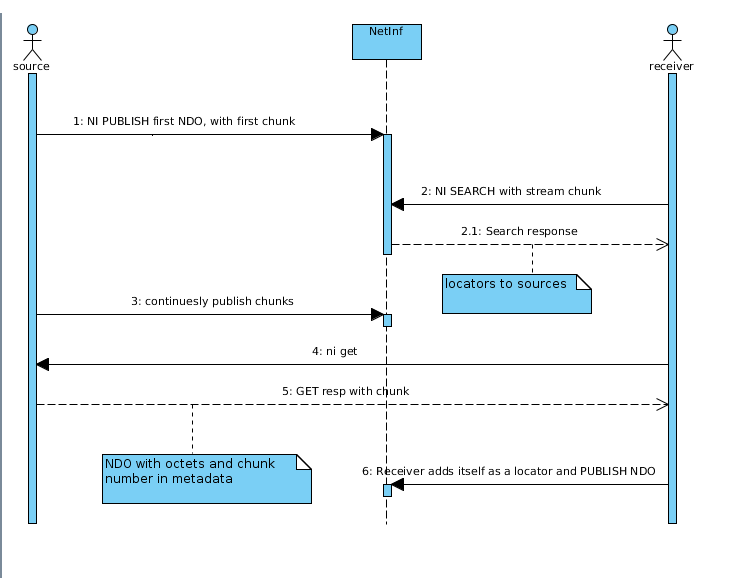
\includegraphics[width=0.75\textwidth]{./img/sequence_diagram_pure_streaming.png}
    	\caption{Chunked Data Transfer With Pure NetInf}
	\label{fig:stream-seq-pure}
\end{figure}

\subsubsection{Streaming Frontend}
To merge the chunks, a simple HTML5 frontend was created. HTML was chosen to make the player platform independent.
In both implementations the player starts a JavaScript that continuously polls the local NetInf node for the chunks through the HTTP dispatcher.
The difference is that the pure NetInf player uses the NRS search to build the playlist, while the modified NetInf version only increases the chunk number.


\chapter{System Architecture}
\label{sec:architecture}

\definecolor{javared}{rgb}{0.6,0,0} % for strings
\definecolor{javagreen}{rgb}{0.25,0.5,0.35} % comments
\definecolor{javapurple}{rgb}{0.5,0,0.35} % keywords
\definecolor{javadocblue}{rgb}{0.25,0.35,0.75} % javadoc

\lstnewenvironment{code}[1][]%
	{\minipage{\linewidth} 
		\lstset{language=Java,
			basicstyle=\ttfamily,
			keywordstyle=\color{javapurple}\bfseries,
			stringstyle=\color{javared},
			commentstyle=\color{javagreen},
			morecomment=[s][\color{javadocblue}]{/**}{*/},
			numbers=left,
			numberstyle=\tiny\color{black},
			stepnumber=1,
			numbersep=10pt,
			tabsize=4,
			showspaces=false,
			showstringspaces=false}}
	{\endminipage}

\section{NetInfService}
\label{sec:NetInfService}

NetInfService is the first of two Android applications. It provides a NetInf node which can be accessed through a RESTful API. This allows any application running on the same device as the NetInfService to access NetInf functionality through simple HTTP requests. The interface is described in detail in Section \ref{sec:RESTful API}. NetInfService is based on the work done in a previous master thesis \cite{masterthesis} and uses and extends OpenNetInf to provide this functionality. An overview of the design of NetInfService can be seen in Figure \ref{fig:netinfserviceoverview}, the individual components are described below.

\begin{figure}[h!]
	\centering
		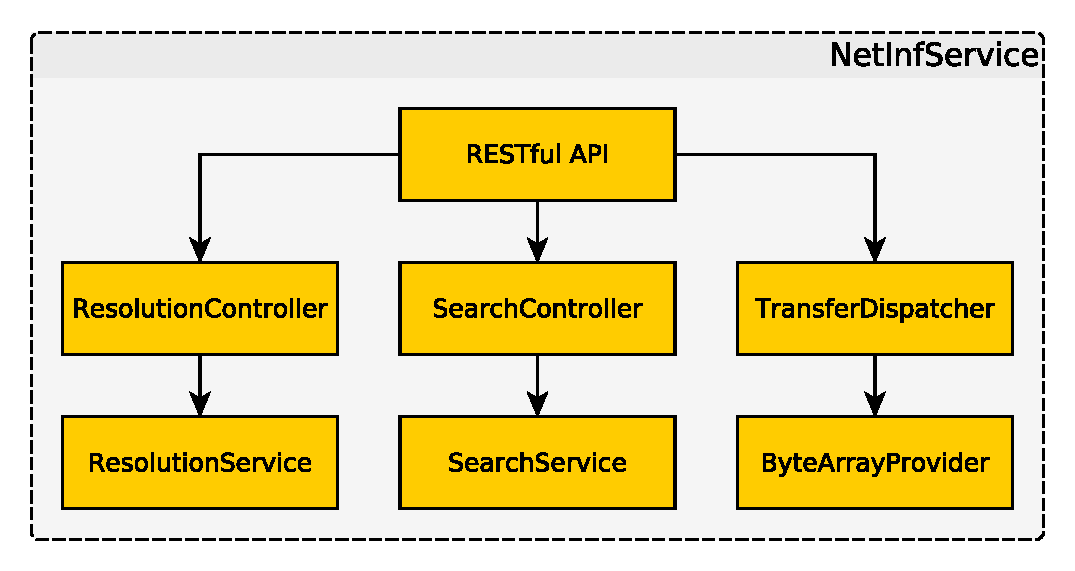
\includegraphics[width=0.75\textwidth]{./img/netinfservice}
    	\caption{NetInfService Overview}
	\label{fig:netinfserviceoverview}
\end{figure}

\subsection{Configuration}
\label{sec:Configuration}

The default settings for NetInfService are stored in the properties file "assets/config.properties". This includes but is not limited to NRS IP address, NRS port, and RESTful API port. Some of these settings can be changed live when running the NetInfService on an Android device. This does not change the default values in the properties file but the changes are instead stored using the default Android shared preferences file, which is persistent.

\subsection{RESTful API}
\label{sec:RESTful API}

The RESTful API receives HTTP requests for NetInf functionality. Depending on the type of request the ResolutionController, SearchController, or TransferDispatcher is called. Publish requests are handled by the ResolutionController. Retrieve requests first do a get using the ResolutionController and then, if the get response contained locators, transfer the file using the TransferDispatcher. Search requests are handled by the SearchController.

The HTTP request use the following format:

\begin{center}
http://\{Host\}:\{Port\}/\{Prefix\}?\{key1\}=\{value1\}\&\{key2\}=\{value2\}...
\end{center}

Since the NetInfService should be running on the same device as the application using it, the host would most likely be either localhost or 127.0.0.1. The default port is 8080, for changing it see Section \ref{sec:Configuration}. The key-value pairs should be URL encoded as they can contain illegal characters.

\subsubsection{Publish}

Publish requests uses the prefix \emph{publish}.

It requires the following key-value pairs:

\begin{tabular}{ | l | l | }
	\hline
	key & value  \\ \hline \hline
	hash & The hash of the object being published.  \\ \hline
	hashAlg & The hash algorithm used to hash the object. \\ \hline
	ct & The MIME content-type of the object being published. \\ \hline
\end{tabular}

The following key-value pairs are optional:

\begin{tabular}{ | l | l | }
	\hline
	key & value  \\ \hline \hline
	btmac & The Bluetooth MAC address of the publishing device. \\ \hline
	meta & Metadata as a JSON string. \\ \hline
	filepath & Path to the file being publish. \\ \hline
\end{tabular}

\begin{itemize}
	\item btmac: The Bluetooth MAC address of the publishing device, it will be added as a locator to the published object.
	\item meta: The metadata for the object that is being published. Remember to URL encode illegal characters.
	\item filepath: The file path of the object that is being published. If this is present a full put is done, otherwise not.
 \end{itemize}

A successful publish returns HTTP status code 200. Any other code indicates something went wrong and should give an indication of what went wrong.

Below is an example of how a HTTP publish request could look like, notice the URL encoding:

http://localhost:8080/publish?hash=TcoP1fQkoxsDq4B8uud\%2Bsyvy0Inu0c7hVLOv7UWN4Nw \\ \&hashAlg=sha-256\&ct=text\%2Fplain\&btmac=f0\%3AE7\%3A7E\%3A3F\%3AD2\%3A43

Unencoded it would look like:

http://localhost:8080/publish?hash=TcoP1fQkoxsDq4B8uud+syvy0Inu0c7hVLOv7UWN4Nw \\ \&hashAlg=sha-256\&ct=text/plain\&btmac=f0:E7:7E:3F:D2:43

\subsection{Retrieve}

Retrieve requests uses the prefix \emph{retrieve}.

It requires the following key-value pairs:

\begin{tabular}{ | l | l | }
	\hline
	key & value  \\ \hline \hline
	hash & The hash of the object being published.  \\ \hline
	hashAlg & The hash algorithm used to hash the object. \\ \hline
\end{tabular}

A successful retrieve returns HTTP status code 200. The HTTP response should contain a JSON object with two key-value pairs. The key \emph{path} should contain a local file path to the retrieved object. The key \emph{ct} should contain the MIME content-type of the retrieved object. Any other code indicates something went wrong and should give an indication of what went wrong.

Below is an example of how a HTTP retrieve request could look like, notice the URL encoding:

http://localhost:8080/retrieve?hash=TcoP1fQkoxsDq4B8uud\%2Bsyvy0Inu0c7hVLOv7UWN4Nw \\ \&hashAlg=sha-256

Unencoded it would look like:

http://localhost:8080/retrieve?hash=TcoP1fQkoxsDq4B8uud+syvy0Inu0c7hVLOv7UWN4Nw \\ \&hashAlg=sha-256

\subsection{Search}

Search requests uses the prefix \emph{search}.

It requires the following key-value pairs:

\begin{tabular}{ | l | l | }
	\hline
	key & value  \\ \hline \hline
	tokens & The tokens being searched for.  \\ \hline
\end{tabular}

The following key-value pairs are optional:

\begin{tabular}{ | l | l | }
	\hline
	key & value  \\ \hline \hline
	ext & An optional JSON, meant for future extensions. \\ \hline
\end{tabular}

\begin{itemize}
	\item tokens: Currently NetInfService only supports one token. This should be changed to accept a string of space separated search tokens to follow specification.
	\item ext: The ext field is meant for future extensions. It is allowed, but currently ignored.
 \end{itemize}

Below is an example of how a HTTP search request could look like, notice the URL encoding:

http://localhost:8080/search?tokens=http\%3A\%2F\%2Fwww.ericsson.com\%2F

Unencoded it would look like:

http://localhost:8080/search?tokens=http://www.ericsson.com/

\subsection{ResolutionController}
\label{sec:ResolutionController}

The ResolutionController handles a number of ResolutionServices. Each ResolutionServices should provide publish, get, and delete functionality using some convergence layer or equivalent. Currently there are two ResolutionServices, the LocalResolutionService which uses a local SQLite database and the NameResolutionService which communicates with a specific NRS using the HTTP convergence layer.

\subsubsection{NameResolutionService}

TODO

\subsubsection{LocalResolutionService}

TODO

\subsection{SearchController}
\label{sec:SearchController}

The SearchController handles a number of SearchServices. Each SearchService should provide search functionality using some convergence layer or equivalent. Currently there is one SearchService, the UrlSearchService, which provide search functionality using a single string which is assumed to be a URL.

\subsubsection{UrlSearchService}

TODO

\subsection{TransferDispatcher}
\label{sec:TransferDispatcher}

The TransferDispatcher handles a number of ByteArrayProviders. Each ByteArrayProvider should provide functionality to retrieve a file (as a ByteArray) in some way. Currently there is one ByteArrayProvider, the BluetoothProvider, which uses Bluetooth to transfer files from other Bluetooth enabled devices.

\subsubsection{BluetoothProvider}

TODO

\section{Elephant}
\label{sec:Elephant}

Elephant is the second Android application. It is a simple browser which uses NetInf through the NetInfService to cache and share web pages.

The idea behind the Elephant browser is simple. When a traditional web URL is entered into the address bar and you click the refresh button, instead of just downloading the web page from the Internet the browser first tries to use NetInf to retrieve the web page.

This is done by using the NetInfService. For the entered URL and each resource it links to:
\begin{enumerate}
	\item Search for the hash of the URL/resource.
	\item Get the file with the given hash.
	\item Possibly publish the file so that others devices can get the file from this device.
\end{enumerate}

If the search or get fails for any reason, be it a timeout, no matches found or something else, the webpage is downloaded using the Internet.

\subsection{Configuration}

The default settings for Elephant are stored in the properties file "assets/config.properties". This includes but is not limited to RESTful API IP address, RESTful API port, and RESTful API timeouts.

\subsection{Control Flow}
\label{sec:Control Flow}

Figure \ref{fig:controlflow} shows a detailed picture of the control flow of the interaction between Elephant and NetInfService. The picture provides the packages and/or source files that are involved in different parts of the program, as well as some text and arrows describing the control flow.

The NetInfService mainly does its work by passing around Identifiers and InformationObjects (which encapsulates an Identifier).

An Identifier contains information about an InformationObject. The most important pieces of information in these applications are:
\begin{itemize}
\item Hash Algorithm
\item Hash
\item Content-Type
\item Metadata (as a JSON string)
\end{itemize}

InformationObjects can contain attributes. In these applications the only used attributes are locator attributes. More specifically locators pointing to other Bluetooth devices and locators pointing to the local file system.

\begin{figure}[h!]
	\centering
		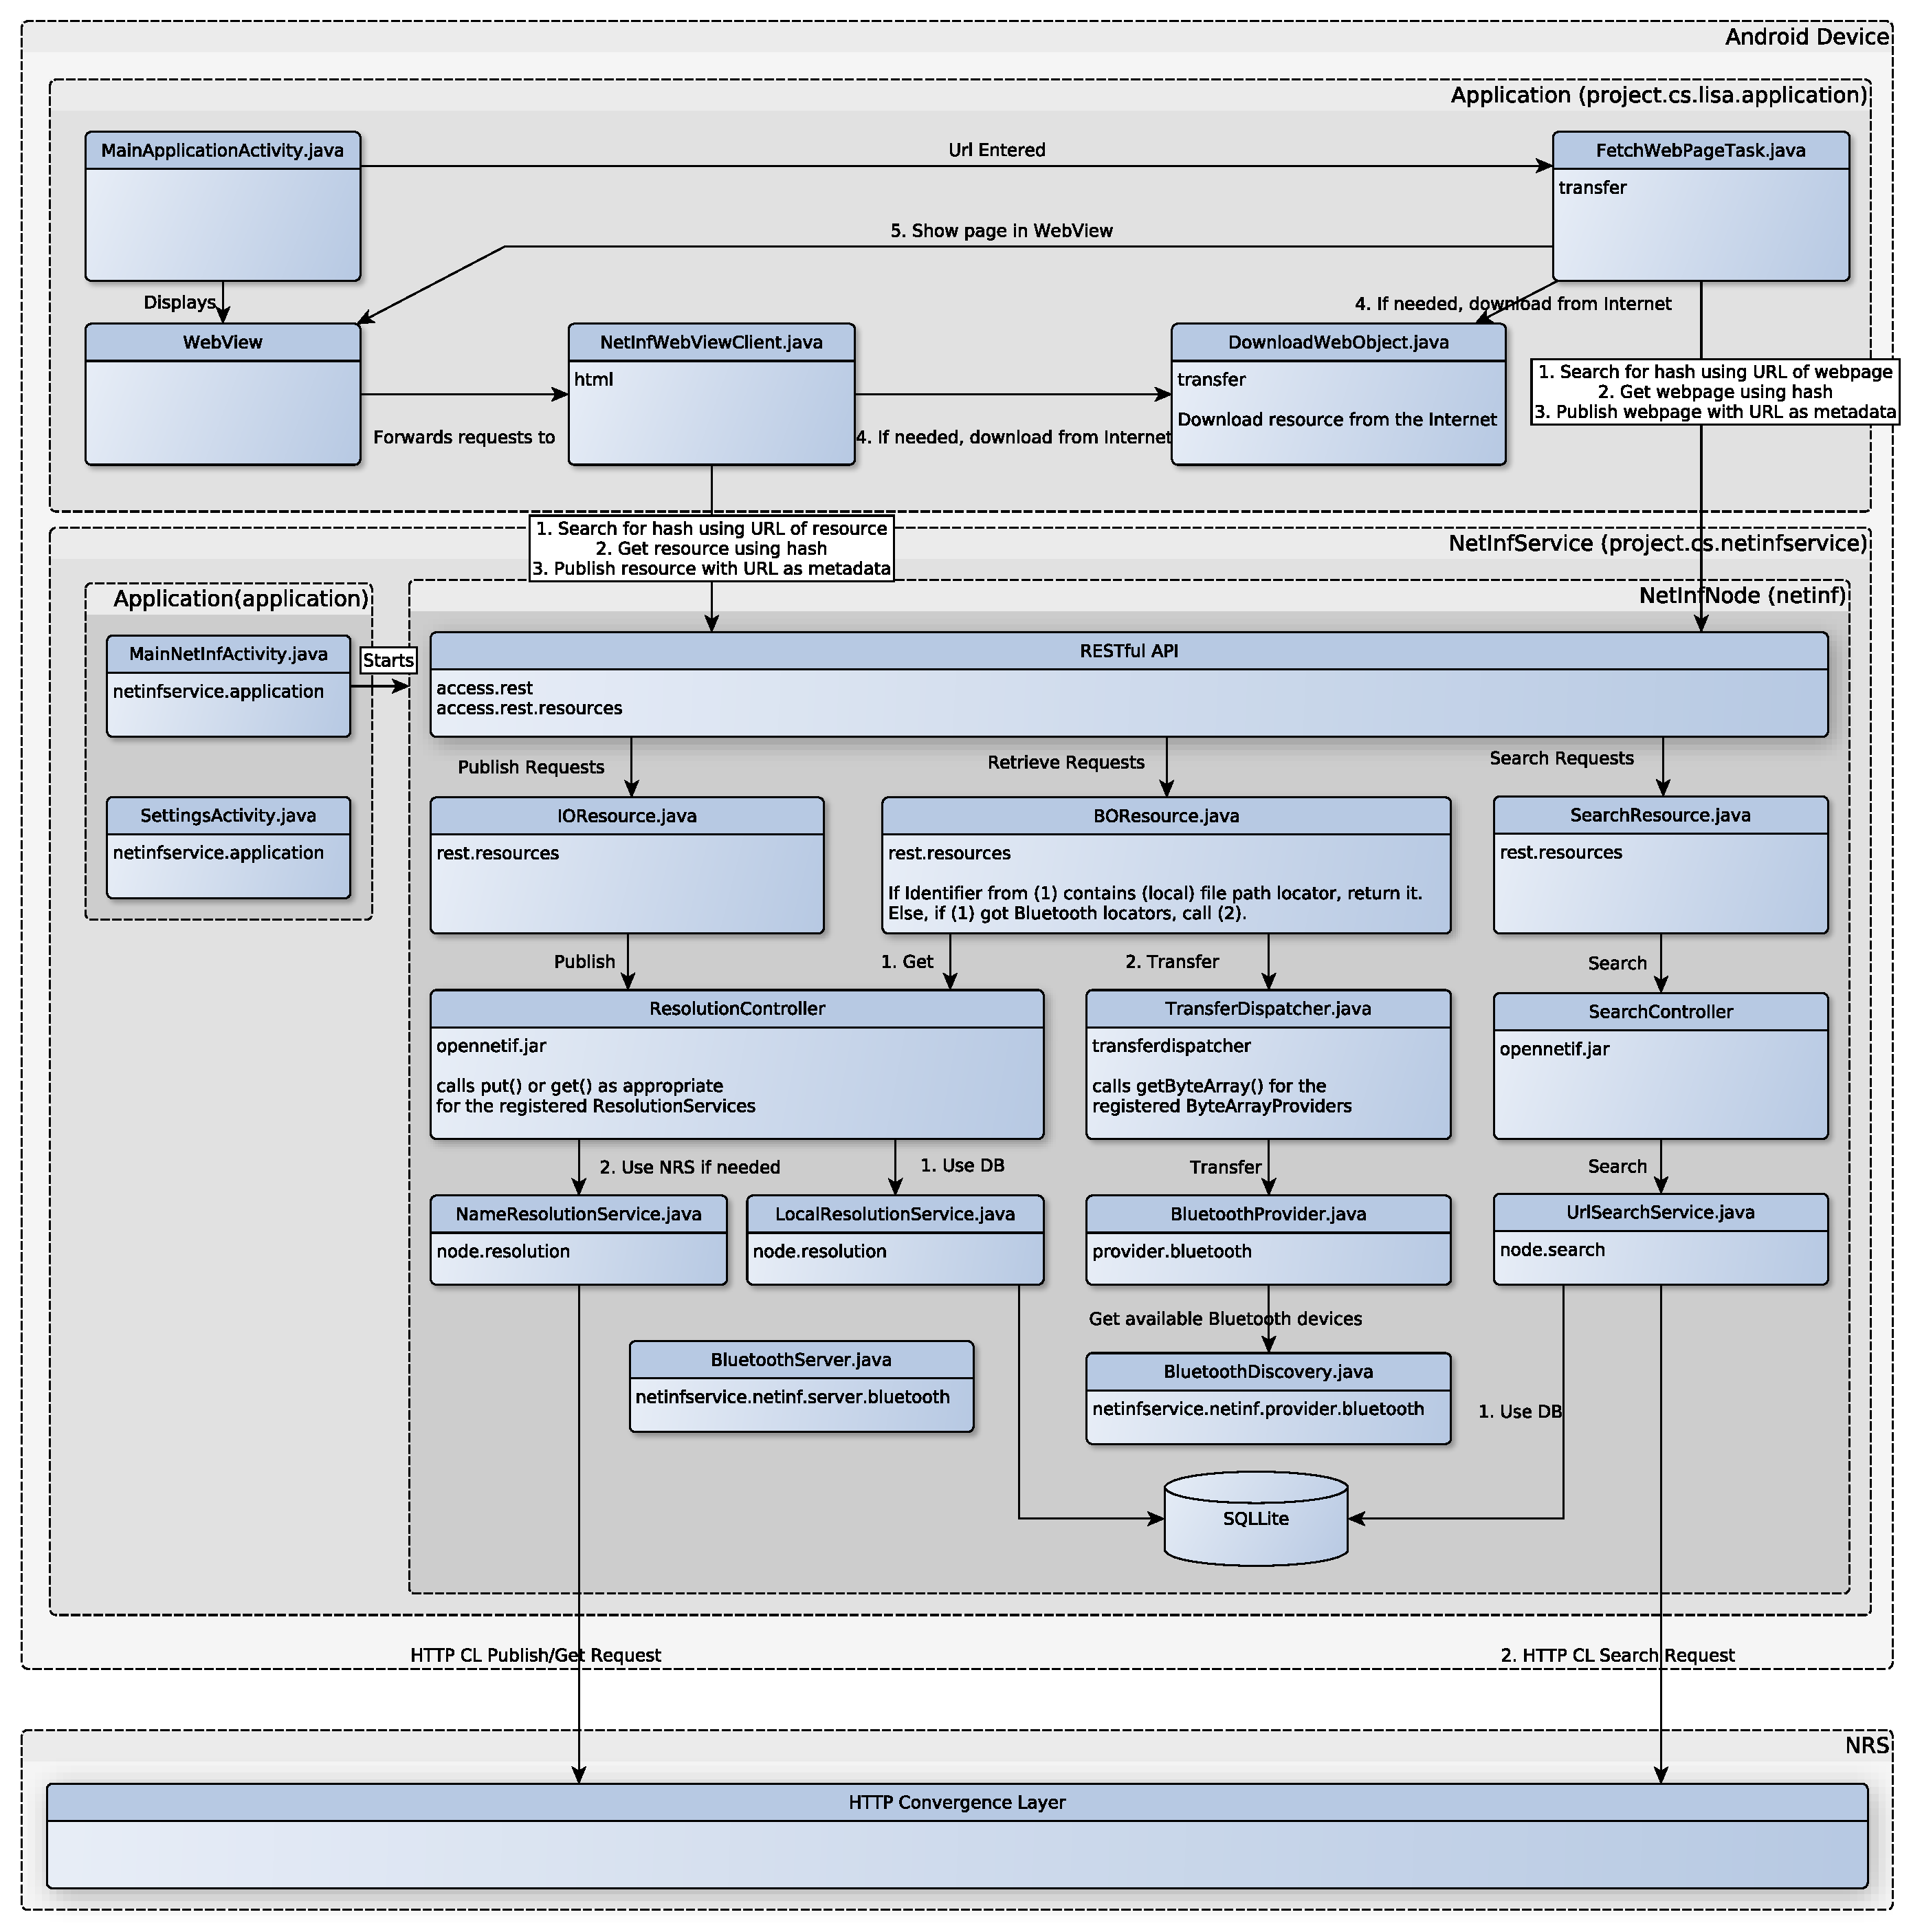
\includegraphics[width=1\textwidth]{./img/flowchart}
    	\caption{Elephant/NetInfService Control Flow}
	\label{fig:controlflow}
\end{figure}

\subsection{RESTful API Access}

Access to the RESTful API is handled by the subclasses of NetInfRequest. There are three subclasses NetInfPublish, NetInfRetrieve, and NetInfSearch corresponding to the API calls for publish, retrieve, and search. NetInfRequest extends the class AsyncTask provided by Android, and hence all subclasses of NetInfRequest are also AsyncTasks.

These classes can be used in two ways. Either by doing a blocking call:

\begin{code}[language=Java]
	// Create a new search
	NetInfSearch search = new NetInfSearch("tokens", "ext");
	// Execute the search
	search.excute();
	// Block until the search response is available
	NetInfSearchResponse searchResponse =
	        (NetInfSearchResponse) search.get();
	// Do things with the response...
\end{code}

Or in a non-blocking way by overriding the function that is called when the response becomes available:

\begin{code}[language=Java]
	// Create a new search
	NetInfSearch search = new NetInfSearch("tokens", "ext") {
            @Override
            public void onPostExecute(NetInfResponse response) {
                NetInfSearchResponse searchResponse =
                        (NetInfSearchResponse) response;
				// Do things with the response...
            }
    }
    // Execute the search
	search.excute();
\end{code}

\section {NetInf NRS}

\section {Overall design}

There are two distinct process types: persistent and non-persistent. The persistent processes will run for the entire uptime of the system whereas the lifetime of a non-persistent process is the duration of its given task. Figure \ref{fig:processhi} below shows the current system design.

\begin{figure}[H]
	\centering
\centerline{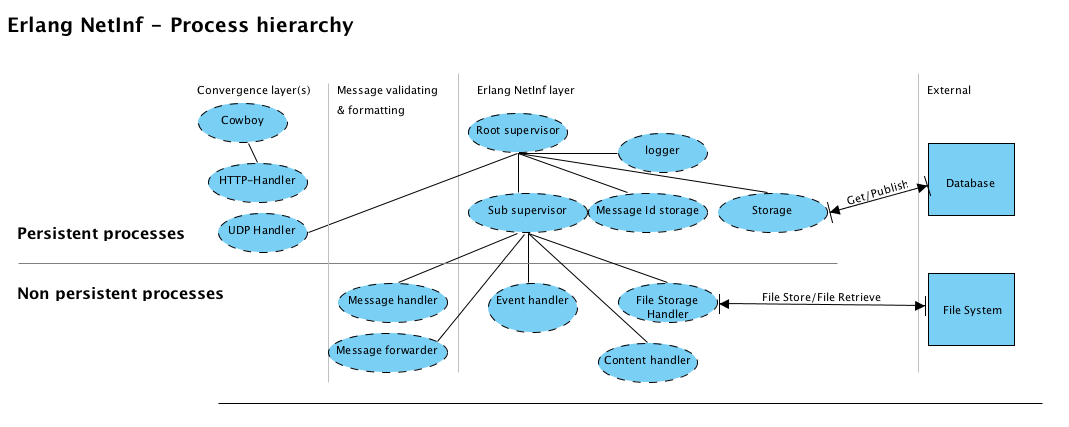
\includegraphics[width=1.2\textwidth]{./img/process_hierarchy.png}}
\caption{Current system design}
\label{fig:processhi}
\end{figure}

\subsection{Architecture layers}

The system architecture is divided into four(4) distinct layers: a network (HTTP, UDP) convergence layer, Message validation and formatting layer, an Erlang NetInf layer and finally an external storage layer consisting of a database as well as access to the file system. Within these layers lie the modules(Erlang processes) which are responsible for specific functions such as sending/receiving convergence layer messages, sanitizing messages, forwarding, accessing databases/file systems and logging.

\subsection{NetInf Messaging}

According to the draft specification(see\cite{netinfproto}) NetInf has three well defined messages which comprise of the core functionality of the system. The following sections describe the purpose and flow of each of these messages in addition to how the Erlang NetInf NRS handles them.

\subsubsection{Named Data Objects}

NetInf describes any piece of information as a Named Data Object(NDO). In the current state of networks, the same piece of information is considered to be host centric and mutable with many copies of the same information lying around. The purpose of an NDO is to provide a convenient way for the protocol to be able to catalogue and preform operations such as storing, retrieving and finally searching for information while eliminating the need for host centric information.

\subsubsection{Internal NetInf Messaging}

The Erlang NetInf NRS uses an internal record to represent a NetInf protocol message. For each request in the system, an instance of the following Erlang record is created and passed to various modules in order to have the specific operation preformed. Afterwards the NRS constructs a response message and sends it back to the requester. There are two records defined in the module nn\_proto, the first defines a request, primarily a Publish, Get, or Search messages from outside of the system(external clients and other NRS'). While the second record defines the NDO. The message record includes the NetInf record (if available). 

\label{NDO-message}
\begin{verbatim}
-record(message, 
	{
	  msgid = undefined :: term(),
	  time_to_live = undefined :: undefined | integer(),
	  octets = undefined :: undefined | binary(),
	  tokens = undefined :: undefined | [binary()],
	  method = undefined :: undefined | get | search | publish | error,
	  netinf = undefined :: undefined | proto() | [proto()] | term()
	}).
\end{verbatim}

The "netinf" field in the above record is dependent on the method and whether or not the message is a request or a response.

\begin{verbatim}
-record(netinf, {
	  % name of the ndo
	  name = undefined :: undefined | binary(),
	  % list of possible locations and or URI's
	  uri = [] ::[] | [binary()], % either empty list or a list of binary terms,
	  % list of extensions stored in json format
	  ext = {[]} :: {[]} | {[{binary(), any()}]}, 
	  % timestamp of the ndo in json format
	  time_stamp = undefined :: undefined | binary() 
	 }).
\end{verbatim}

\subsubsection{Publish}

NetInf describes a Publish message which consists of the following fields:

\begin{description}
\item[URI]  - Contains the hash of the NDO. It is unique to the piece of information that is going to be published into the system. It is also mandatory.
\item[msgid] - A mandatory field as well and it is a unique number(string). 
\item[loc1] - An optional field, this is a locator that can be used to access the information that will be shared.
\item[loc2] - Same as the above.
\item[ext] - An extension field, it is responsible for containing the metadata if any, in JSON format.
\item[rform] - The response format, The NetInf will format the response message using either HTML or JSON. JSON is the default if this field is not set. This is convergence layer specific.
\item[fullPut] - This field is set to determine if octets(binary data) is present with the publish message with either ''true'' or ''false''
\end{description}

\subsubsection{Publish Message Workflow}

\begin{figure}[H]
	\centering
\centerline{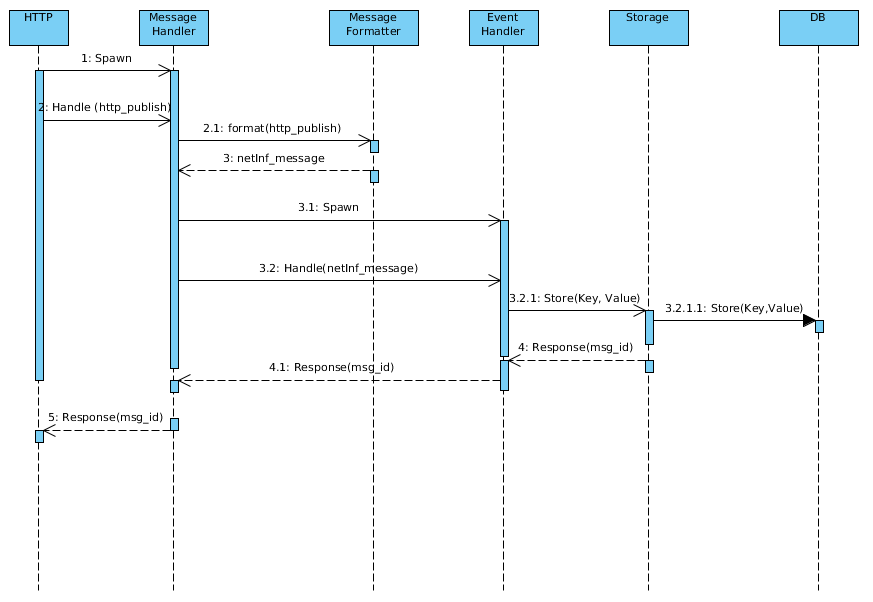
\includegraphics[width=1.2\textwidth]{./img/seq_pub.png}}
\caption{Publish Message workflow}
\label{fig:publishfig}
\end{figure}

A requester would like to share information. Using an external client the requester sends a NetInf Publish Request message with the mandatory fields set as described above through a supported convergence layer(HTTP for example). The Erlang NetInf NRS will then receive the message and create a 'message' record(see section: \ref{NDO-message}).

A convergence layer handler(CL handler) is spawned and receives the request.
Once a request is in the system, the CL handler that received it will pass the request onto the message handler(MH). The MH is independent of the CL however, the formatting library used by the MH will depend on the CL the request was received on.

At this point the original request will be validated and sanitized for use in the internal NRS system and a NDO will be created. If the request is malformed the MH will construct a response message immediately and pass the new message back, informing the requester of the specific reason the request was rejected and then the MH will die. 

In the case that the validation and sanitization succeeds the MH will have a newly sanitized and internal message representation of the original request(NDO). The request is now ready to be passed deeper into the system. The MH spawns an Event Handler(EH) and goes to sleep waiting for the message to complete the process. 

The Event Handler will then read the NDO and determine if a Content Handler(CH) will need to be spawned in order to store the binary data(octets). The CH is only spawned if the FullPut flag in the original request was present and set to 'true'. Finally the EH will pass the NDO to the Storage module and wait until the process is complete.

The Storage module will call the appropriate function for the database(through the functions defined in the Database Wrapper nn\_database). In this case the database will store the published NDO. If a NDO with the same name exists, the two NDO's are merged and the result is stored.

Once the NDO is stored in the database a message is sent back through the chain of waiting processes. This occurs until the Message formatter can create a response containing the NDO that was stored and any CL specific response codes. Note that any process' that were temporarily spawned will kill themselves after the job is complete. Figure \ref{fig:publishfig} shows the flow of communication for Publish requests.  


\subsubsection{Get}

NetInf describes a Get message which consists of the following fields:

\begin{description}
\item[URI] - Contains the unique hash of the NDO as well as the hash algorithm. The user requests the specific data object using this hash.
\item[msgid]- A mandatory and unique number for each message in the system.
\item[loc1] - Same as above
\item[loc2] - Same as above
\item[ext]  - A field reserved for future extensions.
\end{description}

\subsubsection{Get Message Workflow}

\begin{figure}[H]
	\centering
\centerline{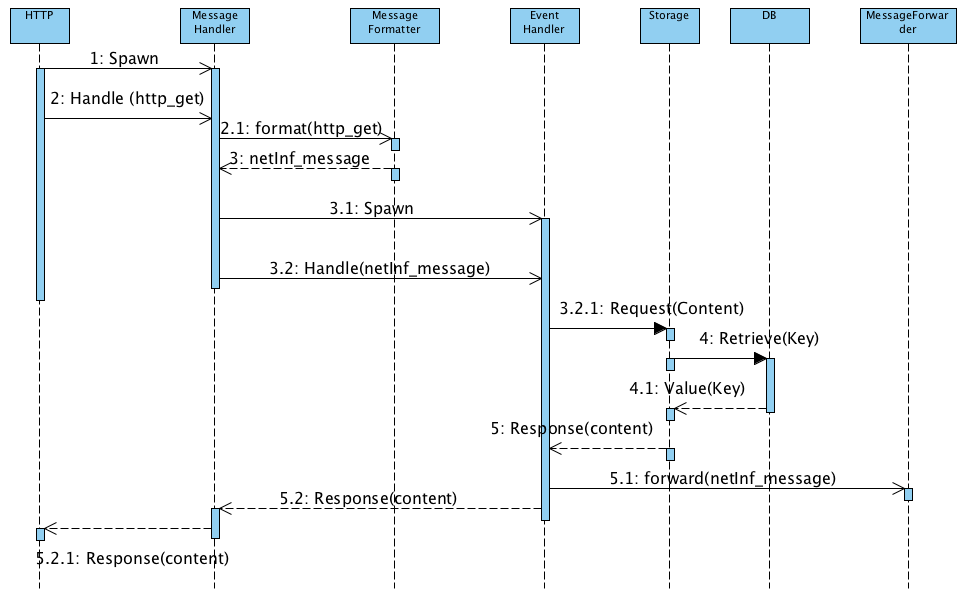
\includegraphics[width=1.2\textwidth]{./img/backend_seq_diagram_GET.png}}
\caption{Get Message workflow}
\label{fig:getfig}
\end{figure}

A requester would like to retrieve information, using an external client the requester sends a NetInf Get request(assuming they know the name of the NDO they are looking for) in the format described above. The process is similar to the publish, until the NDO is passed to the event handler. The event handler will call the database to lookup the NDO using the URI field. If found the NDO will be returnd back through the system to the Message Formatter in order to construct the appropriate response message. However, if the NDO is not found a Message Forwarder will be spawned and the NDO request is broadcasted out on the UDP CL. If there are other Erlang NetInf NRS' on the network a UDP response packet will be sent and the original NRS which forwarded the request will eventually respond to the requester with the NDO or timeout. Figure \ref{fig:getfig} shows the flow of communication for Get requests.

\subsubsection{Search}

NetInf describes a Search message which consists of the following fields:

\begin{description}
\item[msgid] - Mandatory and a unique number.
\item[tokens] - Space delimited text. This is the text that the user will search for within the system
\item[rform] - Optional and will default to Json if not specified, however this is convergence layer specific.
\item[ext] - A optional field reserved for future extensions.
\end{description}

\subsubsection{Search Message Workflow}

\begin{figure}[H]
	\centering
\centerline{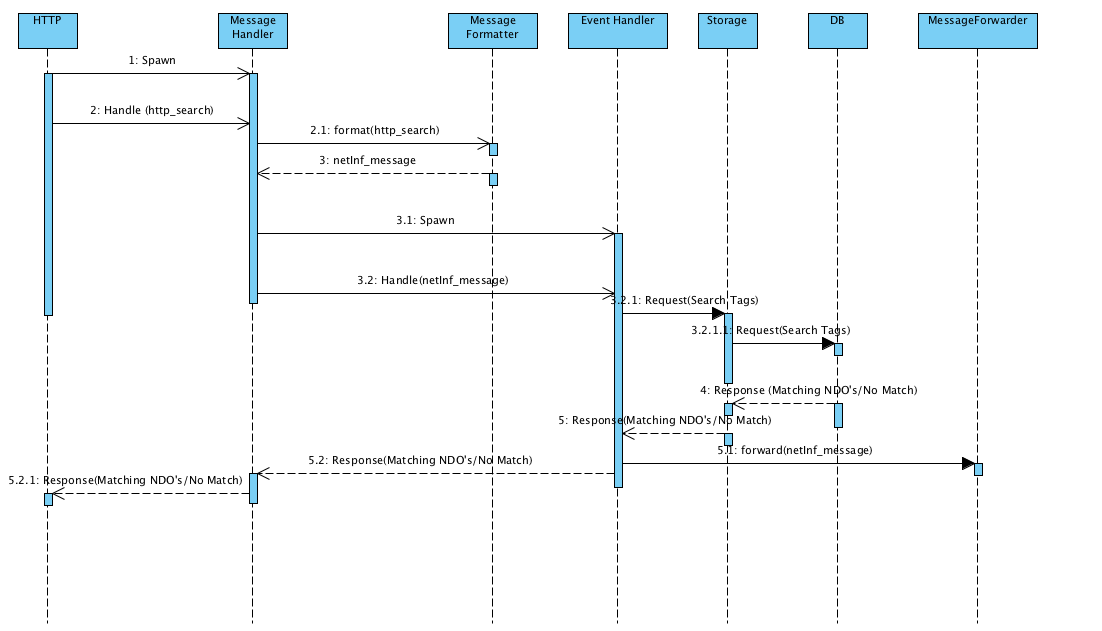
\includegraphics[width=1.2\textwidth]{./img/backend_seq_diagram_SEARCH.png}}
\caption{Search Message workflow}
\label{fig:searchfig}
\end{figure}

A requester would like to retrieve information but they do not know the name of the NDO. A NetInf search request can be sent to the Erlang NetInf NRS to retrieve a list of NDO names and the metadata which match a particular criteria(search tokens). The process is similar to both the Get and the Publish however the event handler calls the appropriate search function in the attached database. If no match is found the request is automatically forwarded on the UDP CL where the same procedure takes place. If a match is found, a response is created  and sent back to the original CL handler. Figure \ref{fig:searchfig} shows the flow of communication for  Search requests.


\newpage
\subsection {Dependencies}

The system architecture for the backend relies on a few external libraries. The following are important for the system to run well. 

\begin {enumerate}
\item Erlang Cowboy \cite{cowboy}

Erlang Cowboy is a small light-weight HTTP server and library written in Erlang for the purpose of handling HTTP requests. The Erlang NetInf NRS product uses functions in Erlang cowboy to communicate with the HTTP convergence layer. Erlang cowboy is responsible for all the multi-part and HTTP requests that are created in the system. 
\item Erlang RTS \cite{erlang}

Erlang Runtime application system is the core Erlang system. Erlang NetInf NRS would not run on the computer system without the core part of Erlang.

\item Erlang covertool \cite{covertool}

Erlang covertool is an Erlang library created by Ivan Dubrov in order to convert the Erlang "cover" reports into a specific format called cobratura XML. This is required for compiling code metric reports and passing them into Jenkins for display on the build server. 

\item Erlang JSON library \cite{json}

Erlang JSON is a library created by Yamashina Hio and Paul J. Davis. This library contains functions which allow Erlang to convert data structures to JSON data structures. The Erlang NetInf NRS uses this library extensively to support storing, retriving and manipulating data in JSON format.
\item Riak \cite{riak} - with search hooks and a Key-Value(KV) bucket installed.
		(Only used for using the system with Riak database)
		
Riak is an open-source scaleable and distributed Erlang database. Created by Basho Technologies, The NetInf NRS uses this database when run with the Riak Database option. Riak was chosen because of it's ease of use and recommendation by the customer. It is the only 'real' database that is currently supported since the other 'database' shipped with the product is an Erlang list data structure.
\end {enumerate}


\subsection {Configurations}

Since the system is supposed to be modular, we have also implemented configuration files. 

Configuration files allow the user of the system to quickly start it with a predetermined setup, things such as which database to use, which convergence layers are supported, and timers for various functionality are also stored here for quick use and editing. The benifit of using erlang specific configuration files is the great way they are organized, giving you a highly readable and easy to swap out functionality. 

We have created 2 config files which live in the root netinf\_nrs directory.

\begin {itemize}
\item list.config
\item riak.config
\end {itemize}

For new databases we encourage a new configuration to be make in order to keep things simple.


The following is the syntax for a config file 

\begin {verbatim}
[{netinf_nrs,
	[
	{key1, value1},
	...
	{keyN, valueN}
	]
}].

\end{verbatim}
And here is an example of how our config file's looks
\begin {verbatim}
[{netinf_nrs,
	[
	{database, nn_database_riak},
	{convergence_layers, ["http"]},
	{ip_timer, 5000},
	{discovery, on},
	{nrs_port, 9999},
	{ct_port, 8078},
	{client_port, 8079}
	]
}].

\end{verbatim}

\subsubsection {Meaning of the config values}
\begin{description}
\item[database]
This is used to define what database to use. The value must be the name of a module that implements our nn\_database behavior. Default is our riak implementation
\item[convergence\_layers]
Deprecated. This was used to define which convergence layers the node should support. Currently we use udp multicast instead
\item[ip\_timer]
Deprecated. This was used to define how often the node broadcasted that it was live to other nodes via udp multicasts
\item[discovery]
Deprecated. This was used to turn of the nodes discovery service for testing purposes
\item[nrs\_port]
This defines what port the NRS will use to listen for NetInf messages
\item[ct\_port]
\underline{\textbf{TODO MARKUS FIX THIS SHIT}}
\item[client\_port]
\underline{\textbf{TODO MARKUS FIX THIS SHIT}}
\end{description}

\subsection {Using config files}

We now need to have a flag on the erl command line that specifies the name of the config file to use. 

\begin {verbatim}
 erl -pa ebin deps/*/ebin -config configs/list
\end{verbatim}

OR

\begin {verbatim}
 erl -pa ebin deps/*/ebin -config configs/riak
\end{verbatim}

Special note: if the netinf\_nrs.app.src file has some configuration options in the env section and there is a config file specified on the erlang command line then the parameters in the config file  will take precendence.

\subsection {Extracting the config parameters}

In the erlang code we use the following 

\begin {verbatim}
application:get_env(app-name,parameter-name) 
\end{verbatim}

where app-name is the name of the application, in our case netinf\_nrs, and parameter-name is the name of one of the parameters defined in the config file OR the env section of the netinf\_nrs.app.src file.

for example to get the database:

\begin {verbatim}
application:get_env(netinf_nrs,database) 
\end{verbatim}

would return {ok, nn\_database\_list} or {ok, nn\_database\_riak} depending on the configuration. 


\subsubsection  {Erlang config files}

for more information see: http://www.erlang.org/doc/man/config.html


\subsection {Convergence Layers}
\label{CL}
The NetInf NRS protocol introduces the concept of Convergence Layers(CL). CL's are specific protocols that can be used to talk to other nodes on the network. For example it is possible to use the HyperTextTransferProtocol(HTTP), Erlang Messaging or User Datagram Protocol(UDP). The CL's are implemented as a set of Erlang modules whose sole jobs are to receive and send messages of the specific type of the CL. These modules receive(CL handlers) clean/format(CL specific formatter) and forward into and out of the system.

\subsubsection{HTTP}

The NetInf protocol draft discusses using HTTP as a primary layer of communication between nodes. All requests on this layer are arriving into the system as HTTP messages and then subsequently changed into internal NetInf Messages. The HTTP CL consists of three(3) modules. 

\begin{enumerate}
\item nn\_http\_handler - uses Erlang cowboy to receive and send HTTP requests to/from the system
\item nn\_message\_handler - Specifically spawned with the attached HTTP formatter in order to process requests
\item nn\_http\_formatting - Handles converting requests/responses from HTTP to NetInf messages and vice versa.
\end{enumerate}

\subsubsection{UDP}

The protocol draft lists it as a CL, however its function is more like a discovery protocol for other NRS' of any type of implementation. The current UDP CL broadcasts NetInf Messages on the network on a multicast IP 225.4.5.6 and port 2345. 

The UDP CL is called when the NetInf NRS receives either a Get or a Search request from some other convergence layer and the requested NDO is not in the the NRS. The Forwarding module will forward the request using the multicast address. Similar to the HTTP CL, this layer consists of three(3) modules as well. 

\begin{enumerate}
\item nn\_udp\_handler - uses the Erlang gen\_udp library to send/receive UDP messages into and out of the system.
\item nn\_message\_handler - Spawned with the attached UDP formatter in order to process requests.
\item nn\_udp\_formatting - Handles converting requests/responses from UDP to NetInf messages and vice versa.
\end{enumerate}

Once the UDP Get/Search messages are sent out to the network, the system may receive back a response with the details asked for by the original request. The UDP\_handler in conjunction with the nn\_message\_handler(Spawned with UDP formatting) will then extract the details, create an internal NetInf Message and forward the message to the process that is currently waiting on the original request. In the case of an HTTP CL, the NetInf message would be forwarded back to the process which deals with the HTTP CL formatting/message handler.

Currently UDP Get and UDP Search requests are supported. The framework for UDP Publish requests are included in the current code base, but have not been used for the purpose of forwarding publishes. 

\subsection {Notes on other CL}

There was a plan to include an Erlang specific CL, this would become a group of modules( handler, formatter) which deal only with Erlang specific messages. However this was a thought that later turned out to be of no real benefit, but extending the system to include this or other CL's could be easily done. 


\subsection {Plug N' Play Database Wrappers}
\label{PNP}
The Erlang NetInf NRS includes functionality to allow for run-time database switching as well as providing an easy way to add interfaces to existing databases. Currently support for Riak is added, as well as a default Erlang list 'database' implementation. The database interface is designed to be very intuitive to implement. Figure \ref{fig:dbfig} shows the interface.

\begin{figure}[h!]
	\centering
\centerline{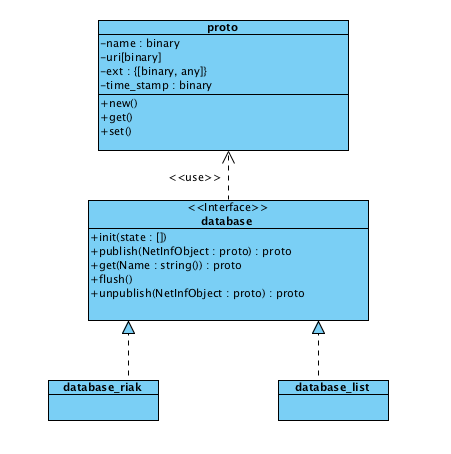
\includegraphics{./img/database_api.png}}
\caption{Database Interface}
\label{fig:dbfig}
\end{figure}

\subsection {Setup of Database Module}

All modules which wish to implement a database connection will use the custom nn\_database behaviour.

\begin {verbatim}
    -module(nn_database).
\end{verbatim}

The following functions must be implemented by all database wrappers

\textbf{Initialization}

\begin {verbatim}
    init() -> 
    	{ok, pid()} | {ok, registered_name:atom()} | {error, string()}
\end{verbatim}

The above function returns the connection for the specified database.
Remember the init should return an identifier to the persistent process of the specified database.

\begin {verbatim}
    publish(NetInfObject::nn_proto:proto()) -> 
    	{ok, ReturnNetInfObj::nn_proto:proto()}
\end{verbatim}

Takes the NetInfObject and returns: \{ok, NewObject\} where NewObject is the NDO created when merging the object being published with an object with the same name in the database. If there was no object with that name in the database, NewObject is the object being published.

\textbf{Get}

\begin {verbatim}
    get(Name::string()) -> 
    	{ok, nn_proto:proto()} | {ok, no_match}
\end{verbatim}

Takes the NetInf Name of the object and returns: \{ok, Data\} where Data is the NDO that was found or no\_match if not found.

\textbf{Unpublish}

\begin {verbatim}
    unpublish(NetInfObject::nn_proto:proto()) -> 
    	{ok, ReturnNetInfObj::nn_proto:proto()} | {ok, no_match}
\end{verbatim}

Takes the NetInfObject and returns \{ok, ReturnNetInfObj\} where ReturnNetInfObj is the NDO entry that was deleted from the specified database.

\textbf{Search}

\begin {verbatim}
    search(SearchList::list()) -> 
    	{ok, list()} | {ok, no_match}
\end{verbatim}

Takes a Erlang list of search keywords and returns a list of the NDO's which match those key words.

\textbf{Flush}

\begin{verbatim}
flush() -> ok
\end{verbatim}

Deletes all the entries in the database.   

Please see the module src/nn\_database\_list as an example of the wrapper implementation for use with a 'list' database in the source code.


\subsection{Chunked data streaming}

The Erlang NetInf NRS includes two different ways to stream chunked data. The first is the modified version of NetInf that removes the overhead of publishing each chunk to the NRS. The other implementation uses pure NetInf to publish each chunk. Both of them use an HTML5 interface to playback the stream. 

%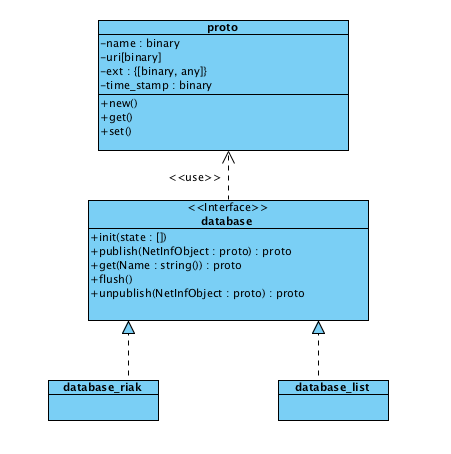
\includegraphics[scale=0.5]{./img/database_api.png}

\subsubsection{Content dispatcher}

To be able to transfer the chunks to the local HTML5 interface a content dispatcher service was added. The difference is that the content dispatcher service serve the NDOs' octects directly through HTTP, that is without the multi-part response as done in the HTTP CL. The module for this is the \textit{nn\_ct\_handler}. This service is spawned when the NRS system starts and runs on port 8078. To request the octects of the NDO \textit{ni:///sha-256-64;abc} pass the url:
\begin{verbatim}
http://localhost:8078/octets/ni%3A%2F%2F%2Fsha-256-64%3Babc 
\end{verbatim}

\subsubsection{Stream handler}
The stream handler module \textit{nn\_stream\_handler} handles fetching and polling of chunked octets between different NetInf nodes. When a user node subscribe to a stream 
In both streaming implementations the logic for fetching the chunks is to shuffle the list of available locators and fetch all available chunks in the ICN. When there are no more chunks, the stream handler retries on a regular interval. After a defined number of retries it will finally terminate itself.  

\subsubsection{HTTP client}
The module \textit{nn\_http\_client\_handler} module is used top serve the HTML5 interface for NetInf Get, Publish and Search requests. It forwards these requests to the local NRS. The client is run on port 8079. The different interfaces that can be seen are

The interface for regular NetInf interaction, located at 
http://localhost:8079/

The modified streaming, located at
http://localhost:8079/stream

The pure streaming, located at
http://localhost:8079/streampure

Other than above viewable URIs there are a couple of other request that can be used to interact with the system. 

Subscribe to a modified chunked stream, http://localhost:8079/subscribe

Subscribe to a pure NetInf stream, http://localhost:8079/subscribe/search\_and\_get


\subsubsection{HTML5 interfaces}
To combine the video chunks, two HTML5 video elements are used to pre-cache the chunks through the transfer dispatcher. This is done by alternating the visibility and playback of the two elements with JavaScript. With this method of playback the chunks looks like one continuous stream. 
To make the usability of the interface smoother, some asynchronous network request are used to communicate with the HTTP client.
To the right of the interfaces it is possible to see the current state of the local NRS. 

\subsubsection{Difference between implementations}


\chapter{Evaluation and testing}
\label{sec:evaluation}
\section{Frontend}

The evaluation of the Elephant browser and the NetInfService applications tries to answer the following two core questions:

\begin{enumerate}
\item How much uplink bandwidth is saved?
\item How much of content is used multiple times throughout web pages?
\item How much of linked resources are dynamically generated?
\item How much time does it take to retrieve web page?
\end{enumerate}

\subsection{Test Setup}

The first test setup consists of a set of web pages from which each of four Android phones will automatically retrieve 15 in a random order. Using the logging functionality of the applications, information about how (Internet, Bluetooth, NRS or Database) resources are retrieved, how many bytes each resource consists of and how long it take to retrieve are acquired. The results are meant to give an idea of the answer to questions 1 and 2.

The web page sets are of sizes 15, 20, 25, 30 and 35. They are derived from the service Alexa \cite{alexa}, which is renowned for its web metrics. This service keeps track of the most visited web sites by country, and the top sites were used to create the sets.

For the backend the setup for the tests consist of a Name Resolution Service that is reset between each test.

The second test setup consisted of first retrieving all web pages from the set of 30 using one phone, and then repeat. The results are meant to give an idea of the answer to question 3. The test is repeated two times. 

\subsection{Hardware}

Tests are run on three Samsung Galaxy Nexus phones and one HTC One X phone using Android OS 4.1.1 Jellybean that were provided by Ericsson.

For the backend the Name Resolution Service was run on a Intel Core 2 Quad CPU Q9400 @ 2.66GHz × 4 with 4 gigabytes of memory using Ubuntu 12.04 LTS.

\subsection{Limitations}

The backend Name Resolution Service supports two types of databases to use for storing published NDOs. The first uses Erlang lists stored in main memory, the other uses a Riak database. The list database was chosen for this test as it is more well tested and easier to work with.

This however means that the test is limited to using the free main memory of the system. A preliminary test using a set of 50 web pages caused the system to run out of memory, resulting in a crash. Therefore, the size of the sets are limited to a maximum of 35 web pages.

\subsubsection{Results}

% Plot of usage

% Table comparing time of access to each resource

% Table (or plot) of re-usage after period

The results of test one can be seen in Figure \ref{fig:frontendtest2}. Each bar represents a specific set size and the colors show how much of the data was transferred with each technology.

\begin{figure}
	\centering
		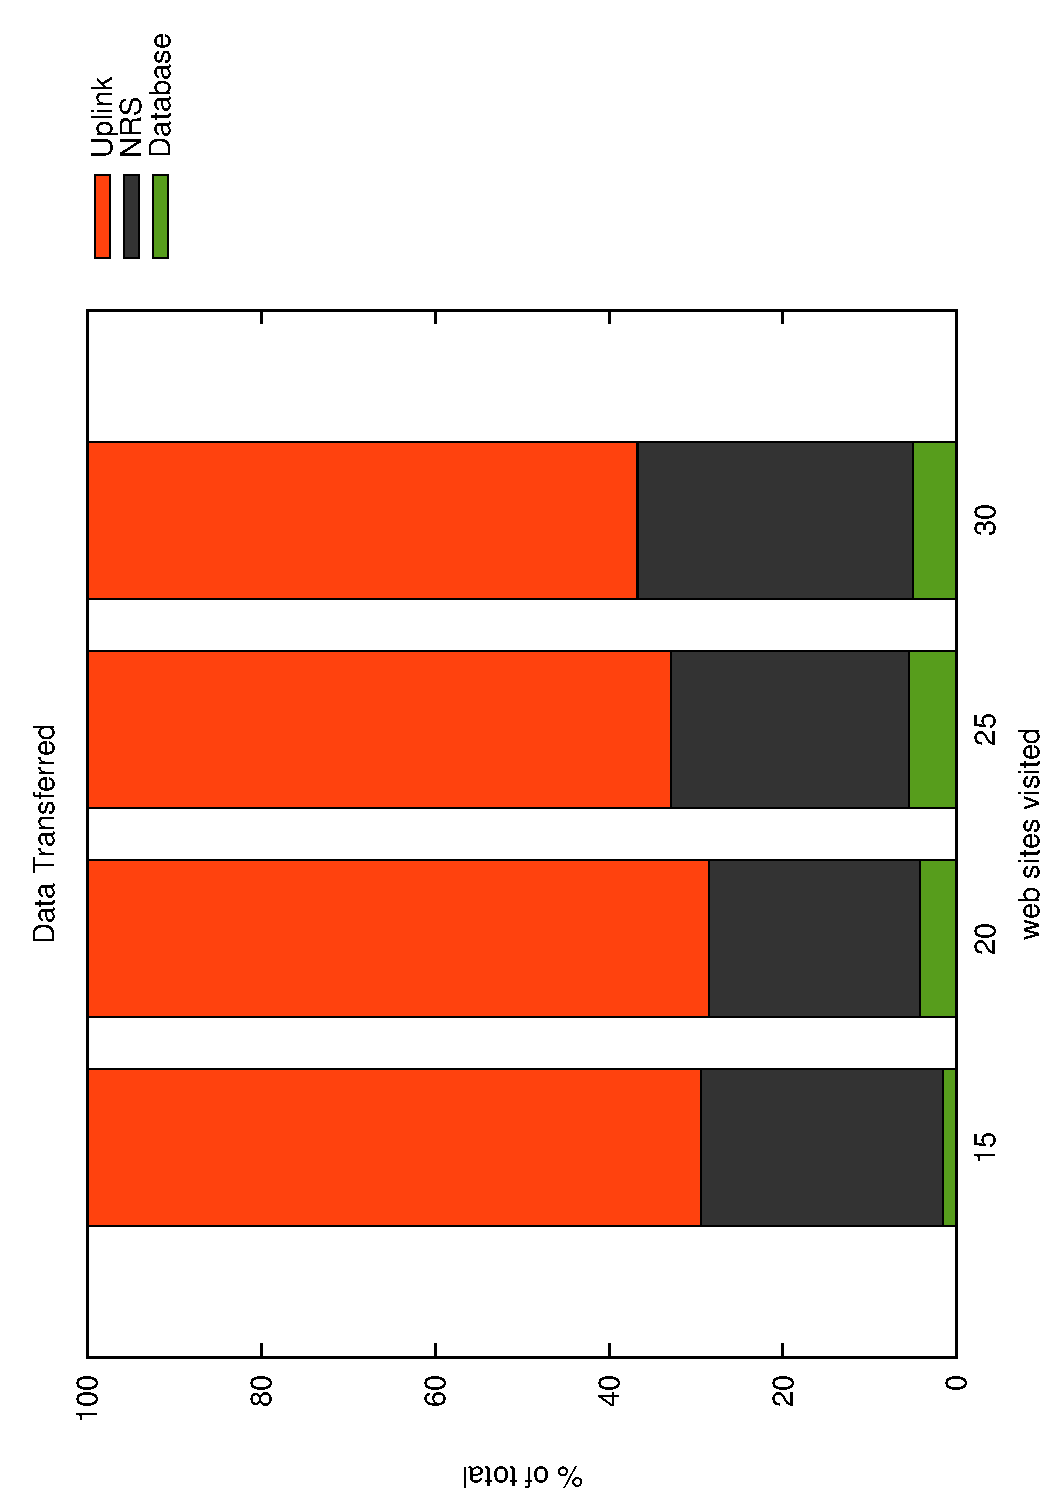
\includegraphics[width=0.75\textwidth, angle=-90]{./img/plots.pdf}
    	\caption{Results of Test 1}
	\label{fig:frontendtest1}
\end{figure}

The results of test two can be seen in Figure \ref{fig:frontendtest2}. The two leftmost bars represent the first repetition of the test and the two right most the second repetition.

\begin{figure}
	\centering
		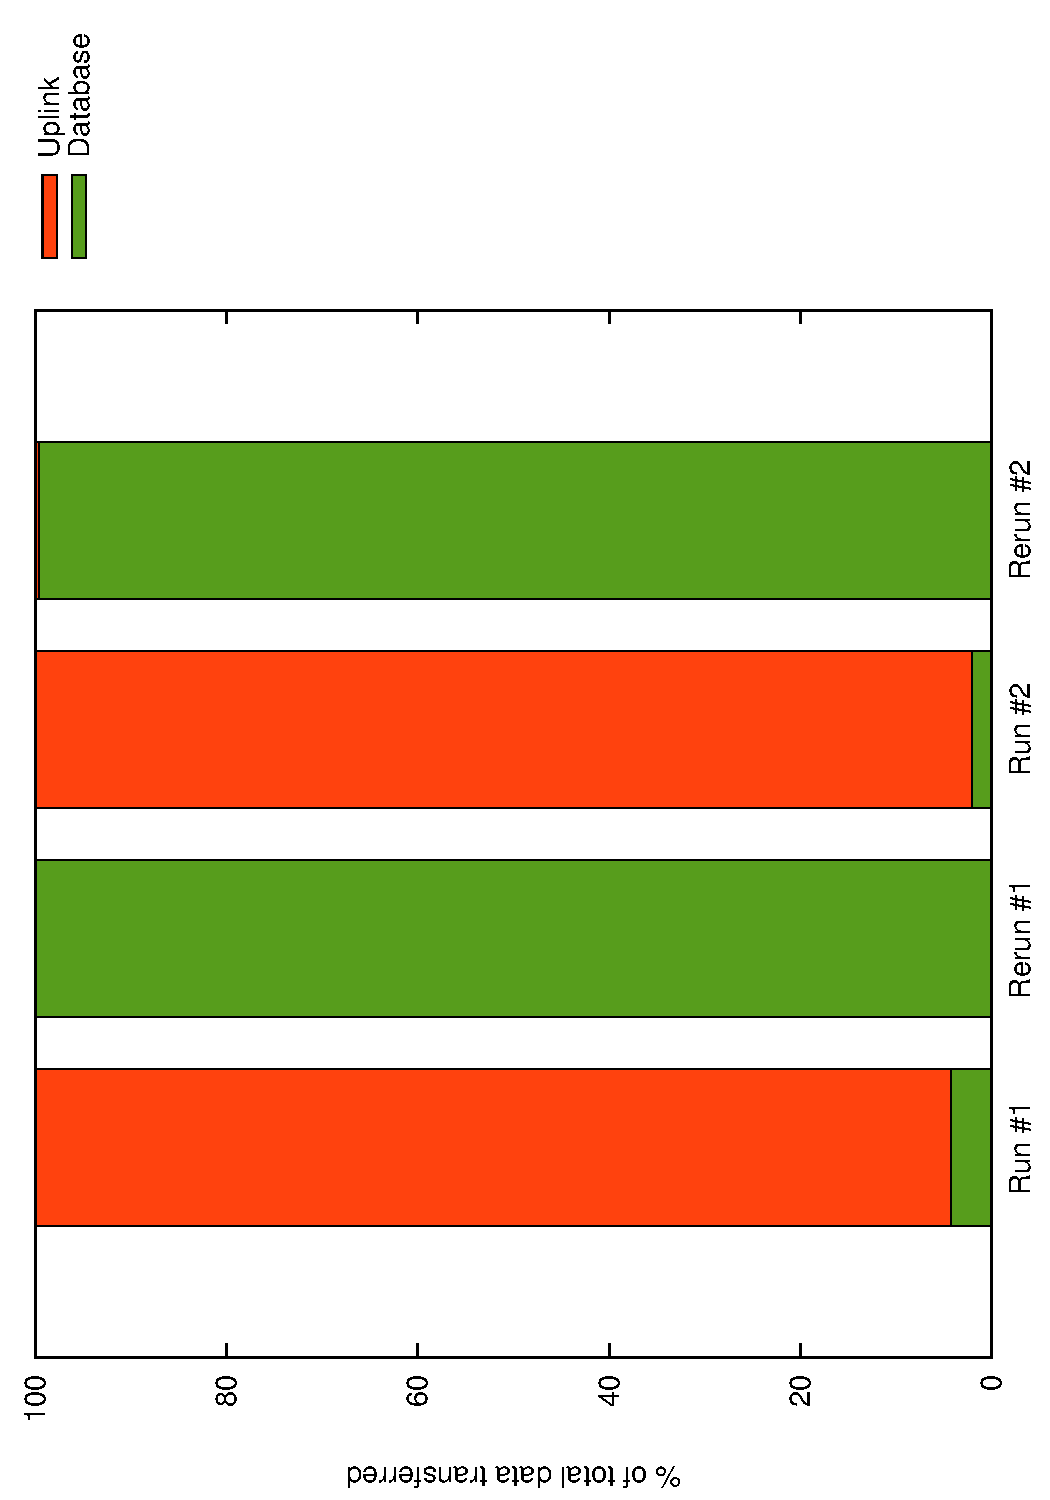
\includegraphics[width=0.75\textwidth, angle=-90]{./img/rerun.pdf}
    	\caption{Results of Test 2}
	\label{fig:frontendtest2}
\end{figure}

\subsubsection{Discussion}

From Figure \ref{fig:frontendtest1}, we can see that even without precaching and even when the phones are not downloading exactly the same web pages, approximately 30\% of the data can be retrieved without using the Internet. With precaching of popular web pages this percentage could possibly increase even further.

One could expect the amount of data retrieved from the Internet to drastically increase as the number of web pages in the set increase since fewer and fewer pages will be retrieved by all phones. This does however not seem to be the case, at least for these set sizes, as can be seen in Figure \ref{fig:frontendtest1}. One possible explanation is that when there are fewer web pages in the set multiple the chance of multiple phones retrieving the same web page at the same time increases. If one phone had a jump start on another phone to start retrieving a certain web page, the second phone shortly caught up with the first phone. The two phones then try to retrieve the same resource at the same time which will not be in the cache and both will use the Internet.

In Figure \ref{fig:frontendtest1} it can also be seen that a few percent of resources are retrieved from the database. This is because these resources are linked to several times throughout the web pages. Since the resource is cached in the database the first time, additional requests can use the database.

From Figure \ref{fig:frontendtest2} we can see that when accessing a web page a second time a small part still has to be retrieved using the Internet. An example of when this can happen is when a web page links to a resource using JavaScript to add a timestamp to the resource's URL. The dynamic nature of this content means that it will not be in any cache when requested. This means there will be a certain amount of resource that will have to be retrieved from the Internet.

From Table TODO REF it can be seen that the retrieval of web pages is very slow. So slow that using this application in a real life situation probably only makes sense if there is no connection at all otherwise. The main culprit behind the long retrieval times seems to be the search. Since a search is done for every web resource the time quickly adds up. To improve the retrieval times of web pages the search needs to be optimized.

One thing that is not immediately visible but that effects the test result is the fact that NetInfService randomly pauses in the background. If this happens it results in all publishes, gets and searches failing which in turn results in everything being retrieved from the Internet. It is suspected that this is caused by how the Android OS handles applications in the background.
\subsection{Backend}

The following section will describe how the NetInf NRS application will be evaluated and tested. One of the goals of the project was to show that the use of the new Network of Information protocol( NetInf) would be better in terms of bandwidth, speed and time compared to existing location based infrastructure. 

The Erlang NetInf NRS application, along with the video stream was evaluated with the following set of tests. 

\begin{description}
\item [Video Streaming protocol evaluation]
The client requested the development team to look into the application of NetInf to real world problems, one of the problems discussed was reducing congestion for broadcasting content(video streaming). 
\begin{itemize}
\item Testing the impure version of NetInf video streaming 
\item Testing the pure version of NetInf video streaming
\item Comparison between both implementations of the NetInf Video streaming
\end{itemize}
\item[NetInf NRS]
The backbone of the entire application, this is the main product which the client requested. It is important to show here just how much better this implementation of NetInf is compared to location based services used today. 

\subsubsection{Notes on Interoperability}

There already are existing implementations done by SAIL and Ericsson Research for the NetInf protocol and in the beginning of the product life-cycle the client requested the development team to try to evaluate the interoperability of this product and others, however as the product evolved the client's requested that the interoperability be left to them to evaluate and for this development team to continue with evaluating the video streaming.

Therefore the development team did not evaluate interoperability at all but there is confidence that with some minor tweaking of the code (due to differences in the various draft versions of the NetInf protocol spec) that this product and others will become interoperable with minimal effort.


\begin{itemize}
\item Evaluation of the search time and get time for the supported databases
\item Resource usage
\item Measuring the number of requests per the frontend phone client
\end{itemize}
\end{description}

\chapter{Conclusions and Future Work}
\label{sec:conclusions}
\section{Conclusions}
The main goals of this project was to develop applications based on the principles of information centric networking using the NetInf protocol. These goals were achieved and the teams were able to build the applications using Java and Erlang/OTP. The backend product(NetInf NRS) is a concurrent and fault tolerant application as per the principles of OTP. Both teams had clear goals when they started the project and achieved it comfortably in the end. Infact, the backend team added functionality to support streaming videos using the application. This functionality was not part of the original plan but because the team achieved all the other major goals well before time.

Both front-end and back-end teams performed testing and evaluation of the application. The back-end team evaluated the streaming with pure NetInf messages and the modified version of streaming based on the draft. Other results that the back-end team observed during the evaluatuion of streaming was that the list database is very slow. This is because the search time is T*N where T is the number of search tokens and N is the number of meta data attribute stored. But as mentioned in the future work section, some other database should be implemented to see if the application works better. In the modified version of streaming we can improve the polling strategy to transfer all the chunks faster. Also the content validation is disabled in the modified version of video streaming and that can cause unauthorized content to be published. The front-end evaluation showed that apart from two problems the application seems to be working as expected. The first problem is the slow searches, which is mentioned above. The second is the problem with NetInfService randomly pausing, which might result from how the Android OS handles background applications.

 

\section{Future Work}

TODO Future Work\\


\chapter{Appendix A: Installation instructions}
\section {Frontend}
This section will describe how to configure the environment to run the frontend application on an Android device. 
This description includes configuring Eclipse with Android in order to continue development. 
The guide assumes that the Java SDK is installed.

The frontend team have been working with:
\begin{itemize}
\item Eclipse Indigo, Service Release 2
\item Android Version 4.1, API Level 16
\end{itemize}

\subsection{Configuring Eclipse with Android}
There are two ways to set up Eclipse with Android.
If Eclipse is installed, follow
the instructions "Installing the Eclipse Plugin" 
at \cite{android} in order to configure the 
Android support for the Eclipse environment.

If Eclipse is not installed yet, Android has released a Bundle that contains Eclipse and all 
necessary tools for developing Android applications.
This bundle can be found at "Get the Android SDK" at \cite{android}.

\subsection{Installing and debugging the application}
The latest version of the frontend code can be found on Github \footnote{Project CS Frontend application. \url{https://github.com/project-cs-2012}}.

In order to run the application on an Android device, connect the device
to a computer, import the project and simply run it in Eclipse. 
Eclipse should recognize the device on its own and immediately offer a list
of available devices, on which the application can be installed on.

For debugging, USB debugging on the device must be enabled.
This setting can be found under the settings menu of the device.

Note that the system might not detect some devices. This issue occurred with
using the HTC ONE x. In that case, a preliminary set up needs to be done.
This set up includes creating a \textit{udev} rules file. More information
can be found under \textbf{"Setting up a Device for Development"} at
\cite{android}.




\section {Backend}
This section describes how to install/setup the Netinf NRS and the NetInf Streaming on a server, it is intended for both end users and developers.

\subsection{Dependencies}

In order to run the system properly the following components are required to be installed on the system, the user can either run the script from the section below, or install these manually.

For the NetInf NRS system:
\begin{itemize}
\item Make
\item Rebar
\item G++ compiler
\item Erlang - version R15B03
\end{itemize}

For the NetInf Video Streaming, in addition to the above the following component(s) are required
\begin{itemize}
\item Google Chrome Web browser - or any other browser that supports HTML 5 video tag.
\end{itemize}

To install Make and G++ manually please run the following commands in the terminal.
\begin{verbatim}
sudo apt-get install build-essential
sudo apt-get install g++
\end{verbatim}

To install Rebar and Erlang manually please follow the following steps

Download and install: Rebar from Github
https://github.com/basho/rebar/archive/master.zip

unzip the archive and run the following command
\begin{verbatim}
 cd rebar-master
 ./bootstrap
 sudo cp rebar /usr/bin
 
\end{verbatim}

To Download and install Erlang - version R15B03.

It can be retrieved from the Erlang-Solutions website or use the following commands.

\begin{verbatim}

wget https://elearning.erlang-solutions.com/couchdb//rbingen_adapter//package_R15B03_precise32_1354121173/esl-erlang_15.b.3-1~ubuntu~precise_i386.deb
 
sudo dpkg -i esl-erlang_15.b.3-1~ubuntu~precise_i386.deb

\end{verbatim}

\subsection{Script}
\label{backend-install-script}
For the convenience of end users and developers, there is a packaged install/setup script available after obtaining the backend code. This script is responsible for quickly installing the entire system with all the dependencies.

\textbf{note if the script is not immediately runnable please run the following command:}
\begin{verbatim}
chmod a+x netinf_nrs.sh
\end{verbatim}

The script can be run by using the following on a command line terminal.

\begin{verbatim}
./netinf_nrs.sh
\end{verbatim}

The script will be put a into a menu loop shown below and instructs the user to type a number in order to choose an option.Choosing an option will preform the task and then cause the script to exit normally.

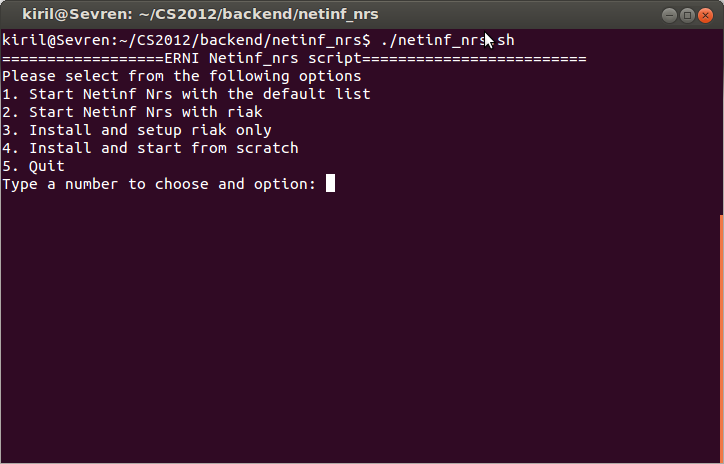
\includegraphics[scale=0.5]{./img/Backend_install_script.png}

The following options are available to the user

\begin{itemize}
\item Start Netinf NRS with the default list\\
Assumes the system has all the dependencies installed and only starts the NetInf NRS with the list database.
\item Start Netinf NRS with riak\\
Will check that Riak is running and present in the system and then start the NetInf NRS with the Riak database.
If riak is not present then the script will download and install all the required components. 
\item Install and setup riak only\\
Use this option only when Riak needs to be downloaded and installed on the machine. This will not start an NRS.
\item Install and start from scratch\\
This option assumes a bare machine and checks that all the dependencies are satisfied. It will auto download and install anything that is required and then start the NetInf NRS with the default list database. 
\end{itemize}


\subsection{Riak Database}

Riak is a database written in Erlang. It is known for being distributed and fault-tolerant. Riak was chosen above other database implementations since it was suggested by the client and the development team had great support available. 

In case there is something wrong with the script process on the target machine please follow the manual installation instructions below.

Install libssl0.9.8 with:
\begin {verbatim}
sudo apt-get install libssl0.9.8
\end{verbatim}

Next install the Riak database:
\begin{verbatim}
wget http://downloads.basho.com.s3-website-us-east-1.amazonaws.com/riak/CURRENT/ubuntu/lucid/riak_1.2.1-1_i386.deb
sudo dpkg -i riak_1.2.1-1_i386.deb
\end{verbatim}

In order for the search to work in the Riak system and from the NRS please enable search.
Riak Search is enabled in the app.config (/etc/riak/app.config) file. Simply change the setting to “true” in Riak Search Config section (shown below).

\begin{verbatim}
%% Riak Search Config
{riak_search, [
               %% To enable Search functionality set this 'true'.
               {enabled, false}
              ]},
\end{verbatim}

Then run the in the terminal;

\begin{verbatim}
riak restart
\end{verbatim}

Followed by the command below to index the bucket:

\begin{verbatim}
search-cmd install netinf_bucket
\end{verbatim}

Lastly, please make sure that the NRS is started with the Riak database.

\subsection{Running the NetInf NRS}

To run the NetInf NRS without the script, please run the following commands after navigating to the netinf\_nrs folder:

\begin{itemize}
\item Using the list database \\
\begin{verbatim}
erl -pa ebin deps/*/ebin -config configs/list -s netinf_nrs 
-eval "io:format(\"NetInf NRS is running ... ~n\")." 
\end{verbatim}

\item Using the riak databse \\
Please make sure the Riak daemon is started before. If it has not been started use the first command shown below before the erl command.
\begin{verbatim}
riak start

erl -pa ebin deps/*/ebin -config configs/riak -s netinf_nrs 
-eval "io:format(\"NetInf NRS is running ... ~n\")." 
\end{verbatim}
\end{itemize}
\chapter {Appendix B: Maintenance instructions}

\section{Frontend}
\subsection{Default Application Settings}

As mentioned in Sections \ref{sec:Configuration} and \ref{sec:ConfigurationElephant} the default settings f
or NetInfService and Elephant are stored in two properties files located at "assets/config.properties" inside each projects folder. 
These files mostly contain internal application settings but also some settings that can be changed through the applications' 
setting menus. If settings are changed through the setting menus 
the default in the files are not changed. Instead the changes are stored using 
the Android concept shared preferences which in short stores the settings in a for each application assigned file.

\subsubsection{Elephant Web Browser}
\label{sec:MaintElephantSettings}

The properties file belonging to Elephant contain the following:

\begin{itemize}
	\item {\bf hash.alg = sha-256}
	
	Constant describing the hash algorithm used. Changing this does not change the algorithm, only the constant used in some functions.
	
	\item {\bf access.http.host = localhost}
	
	The address of the NetInfService RESTful API.
	
	\item {\bf access.http.port = 8080}
	
	The port used by the NetInfService RESTful API.
	
	\item {\bf sharing.folder = /DCIM/Shared/}
	
	The folder used to store downloaded and shared data.
	
	\item {\bf restlet.retrieve.file\_path = path}
	
	The key in the JSON response to a RESTful API retrieve request that contains the file path.
	
	\item {\bf restlet.retrieve.content\_type = ct}
	
	The key in the JSON response to a RESTful API retrieve request that contains the content path.
	
	\item {\bf restlet.search.results = results}
	
	The key in the JSON response to a RESTful API search request that contains the search results.
	
	\item {\bf default.webpage = ul.se}
	
	The default web page of the web view.
	
	\item {\bf httprequest.timeout = 2000}
	
	The maximum time NetInfRequest subclasses wait for a response from the RESTful API.
	
	\item {\bf httprequest.encode = UTF-8}
	
	The encoding is used for HTTP requests.
	
	\item {\bf http = http://}
	
	The HTTP schema.
	
	\item {\bf timeout.netinfsearch = 2000}
	
	Application specific timeout for searches.
	
	\item {\bf timeout.netinfretrieve = 2000}
	
	Application specific timeout for retrieves.
	
	\item {\bf timeout.netinfdownload.webobject = 2000}
	
	Application specific timeout for downloading from the Internet.
	
\end{itemize}

\subsubsection{NetInfService}

The NetInfService properties file contains several settings that are also in the Elephant browser settings. 
Duplicates are not repeated here, instead see Section \ref{sec:MaintElephantSettings}.

\begin{itemize}
	\item {\bf identity.nodeIdentity = ni:HASH\_OF\_PK=123~UNIQUE\_LABEL=456}
	
	The OpenNetInf node identity.
	
	\item {\bf nrs.http.host = 130.238.15.227}
	
	The NRS address.
	
	\item {\bf nrs.http.port = 9999}	
	
	The NRS port.
	
	\item {\bf nrs.http.search.timeout = 20000}	
	
	The timeout when doing a search using the NRS.
	
	\item {\bf metadata.*}
	
	Some field names used as metadata.
	
	\item{\bf bluetooth.interval = 300000}
	
	Period of time, after which a Bluetooth discovery is triggered.
	
	\item{\bf bluetooth.timeout = 10000}
	
	For how long the Bluetooth discover is allowed to run.
	
	\item{\bf bluetooth.number\_attempts = 2}
	
	How many times Bluetooth tries to establish a Bluetooth connection.
	
	\item{\bf bluetooth.buffer = 1024}
	
	The size of the buffer used to retrieve files over Bluetooth.
	
	\item{\bf lrs.priority = 77}
	
	The priority of the LocalResolutionService. Used to determine in which order to use ResolutionServices, higher means more important.
	
	\item{\bf nrs.priority = 42}	
	
	The priority of the NameResolutionService. Used to determine in which order to use ResolutionServices, higher means more important.	
	
	\item{\bf nrs.timeout = 2000}
	
	The HTTP timeout when doing publish or get from the NRS.
	
	\item{\bf nrs.max\_messsage = 100000000}
	
	The maximum number to use as message ID.
	
\end{itemize}

\subsection{Development Environment}

The Elephant browser and the NetInfService applications were developed on Ubuntu using the Eclipse IDE and Android SDK.

For instructions on how to set up Eclipse IDE to use the Android SDK as well as compiling the applications see Section \ref{sec:Frontend Installation Instructions}

\subsection{Eclipse Project Structure}

There are three Eclipse projects:

\begin{itemize} 
 \item Application which contains the code for the Elephant browser
 \item NetInfService which contains the code for the NetInfService application
 \item NetInfUtilities which contain some utility functions used by the two other projects
\end{itemize}
Following are the different packages the applications are structured into and the functionality that is associated with each.

\subsubsection{Elephant Packages}

\begin{itemize}
	\item{\bf project.cs.lisa.application}
	
	Contains the Android Activities for the main view and the settings screen as well as auxiliary code for these.
	
	\item{\bf project.cs.lisa.application.dialogs}

	Contains several popup dialogs either asking for input or displaying information.
	
	\item{\bf project.cs.lisa.application.hash}
	
	Contains SHA-256 hashing functionality.
	
	\item{\bf project.cs.lisa.application.html}
	
	NetInfWebViewClient changes the behaviour of the WebView by telling the WebView what to do
	when new resources are to be downloaded. NetInf is used to search for, download and publish web pages and/or resources. If necessary the Internet is used.
	
	\item{\bf project.cs.lisa.application.html.transfer}
	
	The FetchWebPageTask fetches the HTML source of a web page using NetInf if 
	possible and loads it into the WebView. Then the WebView will load the resources using the NetInfWebViewClient.
	
DownloadWebObject is used be the NetInfWebViewClient to download the web page or resource from the Internet if not accessible by NetInf.
	
	\item{\bf project.cs.lisa.application.http}
	
	Contains the code handling the HTTP communication with the NetInfService's RESTful API. The classes NetInfPublish, NetInfRetrieve and NetInfSearch handle 
	publish, retrieve and search respectively. The classes NetInfPublishResponse, NetInfRetrieveResponse and NetInfSearchResponse represent 
	responses to publish, retrieve and search respectively.
	
	\item{\bf project.cs.lisa.application.networksettings}
	
	Contains code for checking and setting the Android devices network settings properly.
	
\end{itemize}

\subsubsection{NetInfService Packages}

\begin{itemize}
	\item{\bf project.cs.netinfservice.application}
	
	Contains the Android Activities for the main view and the settings screen as well as auxiliary code for these.	
	
	\item{\bf project.cs.netinfservice.database}
	
	Handles the SQLLite database used by both the LocalResolutionService as well as the UrlSearchService.	
	
	\item{\bf project.cs.netinfservice.netinf.access.rest}
	
	Handles the HTTP server providing the RESTful API.
	
	\item{\bf project.cs.netinfservice.netinf.access.rest.resources}	
	
	Contains the implementation of the RESTful API. IOResource handles publish, BOResource handles retrieve and SearchResource handles search.
	
	\item{\bf project.cs.netinfservice.netinf.common.datamodel}
	
	Contains extensions to OpenNetInf NDOs. This includes the metadata and content-type fields.
	
	\item{\bf project.cs.netinfservice.netinf.node}
	
	StarterNodeThread is used to start a NetInf node.	

	\item{\bf project.cs.netinfservice.netinf.node.exceptions}

	The InvalidResponseException is used when an invalid response is returned to a NetInf message.
	
	\item{\bf project.cs.netinfservice.netinf.node.module}
	
	The Module class binds abstract interfaces to concrete class implementations using Guice \cite{guice}.
	
	\item{\bf project.cs.netinfservice.netinf.node.resolution}
	
	The resolution package contains the different ResolutionServices, see Section \ref{sec:ResolutionController}.
	
	\item{\bf project.cs.netinfservice.netinf.node.search}
	
	The search package contains the SearchServices, see Section \ref{sec:SearchController}.
	
	\item{\bf project.cs.netinfservice.netinf.provider}
	
	Contains the ByteArrayProvider class, see Section \ref{sec:TransferDispatcher}.
	
	\item{\bf project.cs.netinfservice.netinf.provider.bluetooth}
	
	The BluetoothDiscover class is used to periodically search for and store nearby Bluetooth devices.
	
	The BluetoothProvider class is described in \ref{sec:BluetoothProvider}
	
	\item{\bf project.cs.netinfservice.netinf.server.bluetooth}
	
	The BluetoothServer listens for incoming Bluetooth pairing requests. As soon as the local device has been 
	successfully paired with a remote device, the BluetoothServer waits for a file request containing a hash. If the specified file is available, 
	the file will be transferred to the remote device.
	
	\item{\bf project.cs.netinfservice.netinf.transferdispatcher}
	
	Contains the TransferDispatcher class, see Section \ref{sec:TransferDispatcher}.
	
	\item{\bf project.cs.netinfservice.util}

	Contains utility classes.
	
	The IdentifierBuilder and IOBuilder classes ease the construction of Identifiers and InformationObjects respectively.
	
\end{itemize}

\subsection{Javadoc}

Javadoc was used during development to document the functionality of classes. For more detailed desciption of classes and their methods refer to the Javadoc.
\section{Backend}
The following section describes the maintenance and default settings of the backend team's NetInf NRS as well as the NetInf Video Streaming.

\subsection{Default Application Settings}

The NetInf NRS application is controlled using one out of two methods, first through the Erlang application src file(netinf\_nrs.app) 
found in the netinf\_nrs/src directory. The second from the configuration files loaded at run time from the configs directory. 

By default the following settings are used when there is no specification on the Erlang command line which config file is to use, 
please refer to section \ref{backconfig} to understand what each setting is used for. 

In short, the Erlang NetInf NRS will be started with the list database.

\begin{description}
\item[database]
nn\_database\_list
\item[convergence\_layers]
["http"]
\item[ip\_timer]
5000
\item[discovery]
off
\item[nrs\_port]
9999
\item[ct\_port]
8077
\item[client\_port]
8079
\item[list\_timer]
3600
\end{description}

\subsection {Development Environment}

To those wishing to continue the development of the Erlang NetInf NRS and the NetInf Video Streaming, the following 
section details how the development environment was set up. 

Please note that the applications were developed on the Ubuntu 12.04 LTS platform, deviating from this may cause the 
application to behave in unexpected ways.

The recommended editor used was Emacs with the erlang-mode, this editor and mode can be installed using the following commands:

\begin{itemize}
\item sudo apt-get install emacs
\item sudo apt-get install erlang-mode
\end{itemize}

Useful emacs commands include:

\begin{itemize}
\item ALT+X \\
Sets up Emacs for the meta-command mode. Erlang-mode can be set by typing
ALT+X erlang-mode
\item CTRL+X+F
Opens a file or create a file. 
\item CTRL+X+S \\
Emacs quick short cut for saving files
\item CTRL+C+K \\
Emacs quick short cut for compiling and saving Erlang files
\item CTRL+X 1-3 \\
Emacs quick short for dividing the windows into 1 whole window(1), horizontally(2) or vertically(3).
\end{itemize}

Please note that Emacs has auto-completion for commands when pressing tab. Other useful tips include Erlang-mode 
skeletons which allow the developer to import comment sections and whole skeletons for generic servers and behaviours.

In addition to running the NetInf NRS, developers should note that Erlang comes with a utility to monitor the processes 
spawned in applications called AppMon. To start AppMon, start an Erlang shell and use the following command.

\begin{verbatim}
appmon:start(). 
\end{verbatim}


\subsection {Code and folder structure}

The NetInf NRS and the NetInf Video Streaming application are organized in the following way:

\begin{description}
\item [netinf\_nrs]
The main folder which holds the following folders as well as the other important files for the application.
\item [configs]
The folder which contains all the configuration files for the NetInf NRS application. Please place all the new configuration files here. 
\item [curludp]
This folder contains a text file which is read by udp\_test.sh. It has no other uses.
\item [deps]
This folder is created automatically by running the rebar (or the script, which invokes makes and eventually rebar). 
It contains all the dependency code required for libraries that were used in the NetInf NRS application. 
\item [doc]
This folder is created automatically by running the rebar doc command (see \ref{bdoc}). Use the index.html file to get to 
the first page of the documentation. Note that this is normally not present unless the doc command has been run.
\item [ebin]
This folder contains all the compiled Erlang beam files, this is where the Erlang virtual machine will look for the compiled code modules.
\item [files]
This folder contains all the stored binary content (NDO cache). The NetInf NRS will look here and determine if it has the content 
or not. If the NRS recieves a get message, alternatively if the NRS receives a publish message with binary octets, it will save it here. 
This folder is required for the NRS to start properly and will be created using the make target "set\_env\_folders".
\item [logs]
This folder contains all the logging files, it also contains a folder named old. The logger service in the NRS will create a text file 
with information about the NRS and current activities up to a default size of 10MB (may be changed in the nrs\_logger.erl file 
in the src directory). This folder is required for the NRS to start properly, this folder will also be created using the make target "set\_env\_folders"
\item [resources]
This folder contains all the resources associated with the HTML client interface for the NetInf NRS video streaming.
\item [src]
This folder contains all the source code for both the NetInf NRS and the video streaming.
\end{description}

Please note that inside the main netinf\_nrs folder several files exists consisting of a Makefile, rebar.config file, udp\_test.sh -udp 
testing script, readme and the netinf\_nrs startup/install script. 

\begin{description}
\item[Makefile]
This is the make file with several targets shown below. It is primarily used for compiling the NetInf NRS project and invoked by the 
main netinf\_nrs script. 
\begin{itemize}
\item all \\
Creates the required folders for the environment, compiles both erlang source code and the JSON c++ and finally runs eunit but this 
does not start the NRS.
\item all\_no\_test \\
Same as the above, however it does not invoke the eunit tests.
\item eunit \\
Runs the eunit tests using the rebar and skips all the dependency tests (only tests NetInf NRS).
\item integration\_test \\
Compiles the Erlang source code and the dependencies if needed and then runs only the integration\_test code.
\item integration\_test\_riak \\
Same as the above but will attach the Riak database to the Erlang NetInf NRS instance and run the integration\_test code on that.
\item makec \\
Compiles only the C++ JSON dependency code in the deps folder. 
\item set\_env\_folders \\
First removes the following required folders: logs and files and then re-creates them.
\item compile \\
First tests if the "deps" folder already exists and then compiles the dependencies, otherwise it will download all the required dependencies 
and then compile them.
\item compile\_deps \\
Cleans the "deps" folder, then downloads all the dependencies again and compiles them.
\item start\_script\_riak \\
Runs the steps in the all\_no\_test target, then starts the NetInf NRS with the Riak database attached.
\item start\_script \\
Runs the steps in the all\_no\_test target, then starts the NetInf NRS with the default list database attached.
\item clean \\
Removes the environment folders (logs and files) and removes the ebin compiled folders as well as the crash dump if the Erlang virtual 
machine has crashed previously.
\end{itemize}
\item[rebar.config]
This file defines all the settings for rebar in this particular product. The dependencies as well as options for eunit and various 
plugins to rebar can be configured.
\item[udp\_test.sh]
This file is a script for testing the UDP convergence layer. Please note that it is best tested with the discovery turned off in the config file. 
At least two different computers are required to run these tests. All instructions are in the script. 
\item[netinf\_nrs.sh]
This file is the main setup/install and run script. Please use this to install all the required components on the machine to ensure 
maximum compatibility. More details about this script can found seen in \ref{backend-install-script}
\end{description}

\subsection {NetInf NRS modules}

The main code modules are located in the "src" directory of the main folder. Each file has comments inside which can be generated into 
documentation please see subsection \ref{bdoc}

\begin{description}
\item[Erlang-application file]
Erlang applications require a definition file in order for the Erlang virtual machine to be able to understand which modules need to be
preloaded and what configurations if any need to be supplied to the application.
\begin{itemize}
\item netinf\_nrs.app.src - This file gets read by the Erlang virtual machine at compile time. Developers can set various options for the 
default settings in the "env" section of the file.
\end{itemize}
\item[Supervisors]
Erlang uses supervisors to organize which process must stay alive for a application to function as intended, below is a brief description 
of all the supervisors required in the NetInf NRS application
\begin{itemize}
\item nn\_sup - This is the main supervisor which starts the persistent processes mainly: sub, msg id, and client supervisors as well as 
the storage, discovery(deprecated), logger, stats and the udp handler.
\item nn\_sub\_supervisor - This is the sub supervisor. It is responsible for starting the following non-persistent processes: event\_handler, 
message\_handler, content\_handler, http\_forwarder, udp\_forwarder and finally the content\_transfer\_handler.
\item nn\_client\_supervisor - This is the client supervisor. It is responsible for starting the http client stream handler. 
\item nn\_msgid\_sup - This is the message id supervisor. It is responsible for starting the modules associated with message id storage.
\end{itemize}
\item[Convergence-Layers]
As stated in section \ref{CL} the application was designed to be modular, the idea of convergence-layers allowed the application to group 
three distinct modules together to create the convergence-layer in Erlang.
\begin{itemize}
\item nn\_http\_handler - This module contains code to process and send/receive http requests from the outside world(using the cowboy library). 
It is the first part of the HTTP convergence layer.
\item nn\_http\_forwarder - This module contains code to send and receive http requests to other NRS' when a search has failed in the NRS system.
Note, this feature(HTTP forwarding) is only used when the system has been started with the static\_peers configuration. See \ref{backconfig} for more details.
\item nn\_http\_formatting - This module is responsible for taking a HTTP message and converting it to the internal representation of the NetInf 
Message and vice versa. It interacts with the message\_handler passing converted messages back and forth. The message\_handler that has been spawned 
with HTTP as the convergence layer uses this module.
\item nn\_udp\_handler - This module contains code to send/receive NetInf UDP messages. It is spawned by the sub supervisor and serves as the entry 
and exit point of the system for the UDP convergence layer.
\item nn\_udp\_forwarder - This module contains code to convert and forward messages from another convergence layer into UDP specific messages and 
then passes them to the UDP handler to send out of the system.
\item nn\_udp\_formatting - This module contains code to convert UDP NetInf messages and extract information into a NetInf Message for use in the 
message\_handler. The message\_handler that has been spawned with UDP as the convergence layer uses this module.
\item nn\_message\_handler - This module is responsible for accepting messages from a convergence layer handler. It is spawned with the specific 
convergence layer name so that the module can redirect requests to the appropriate formatter. The handler also forwards messages to the event 
handler for further processing in the system.
\end{itemize}
\item[Database behaviour \& Storage interface]
This application contains a custom behaviour to allow developers to quickly create wrappers for databases as well as functionality to change the 
database at run-time. The following modules are involved:
\begin {itemize}
\item nn\_database - This is the custom behaviour implemented for creating database wrappers. Each new database wrapper must implement this behaviour. 
Erlang will then warn the developer if there are missing key functions in the implementation of the new database wrapper. The section PNP Database Wrapper 
\ref{PNP} has more information.
\item nn\_storage - This is the interface between the database wrapper and the content caching. This module is responsible for facilitating requests 
from the event\_handler.
\end{itemize}
\item[Databases]
The NetInf NRS application has support for various plug and play database wrappers. As long as the developer adheres to the required input and output of 
the database behaviour this application can be extended to work with any database. 
\begin{itemize}
\item nn\_database\_list - This module implements the callback functions defined in the nn\_database. It is also a quick database consisting of a persistent 
Erlang list data structure. The module also has a timer which causes the list structure to be saved to disk every hour. This can be controlled in the 
configs/list.config file under the appropriate variable.
\item nn\_database\_riak - This module implements the callback functions defined in nn\_database, it is a wrapper for talking to a Riak process (Riak is a standalone database).
\end{itemize}
\item[Content-Caching]
The NetInf NRS also includes a method of caching binary objects sent into the system via NetInf messages, the following are the two modules involved in this functionality.
\begin {itemize}
\item nn\_content\_handler - This module is responsible for handling the binary octets(files) coming into the system it is also the interface for 
storing and retrieving the files associated with NDOs.
\item nn\_hash\_validation - This module validates the hash of the NDO coming in against the one that is currently stored in the files folder. Please 
note that the files folder must be present in the system otherwise the application will crash. As stated previously, the make target "set\_env\_folders" 
can be used to create the required environment folders.
\end{itemize}
\item[NetInf Video Streaming]
The NetInf NRS application supports a video streaming protocol on top of the existing application. The main files used in this protocol are described here. 
Note that the video streaming also relies on the resources folder as well to provide the http client interface to the user. 

\begin{itemize}
\item nn\_subscribe - Responsible for subscribing to a stream, it is only used in the NetInf video streaming.
\item nn\_stream\_handler - Responsible for polling and fetching the chunks for the users.
\item nn\_stats - Responsible for keeping track of various statistics.
\item nn\_ct\_handler - Responsible for transferring of content without NetInf
\item nn\_http\_client\_handler - Responsible for exposing the http\_client\_interface to users.
\item nn\_http\_ct\_handler - Responsible for transferring of content over HTTP.
\end{itemize}

\item[Logger]
The NetInf NRS application supports a file based logging method, which creates a file named log.txt in the logs folder. The logger comes with three(3) 
levels: verbose, warning and error. Developers can choose which level to log at in the configuration file. By default the log file sizes are set to 10MB 
and then the log file gets moved to the old/ folder. You can increase this in the nn\_logger module under the macro LOG\_FILE\_SIZE.
\begin{itemize}
\item nn\_logger - This module is responsible for opening the log file and writing to it.
\item nn\_logger\_server - This module is responsible for handling the requests to log the event from various modules.
\item nn\_log\_handler - This module contains the gen\_event server which the logger modules connect to, the logger server accepts the requests from the handler.
\end{itemize}
\item [Message ID storage]
The distributed nature of the NetInf NRS and multiple messages required the developers to be able to keep track of which message is associated to a 
specific process id and convergence layer handler. The message storage is a persistent table that maps this and allows the application to forward requests to specific handlers. 
\begin{itemize}
\item nn\_msgide This module contains code to store one message id to process id mapping. 
\item nn\_msgids This module contains code to initiate to insert, lookup and delete the message ids
\item nn\_msgid\_store This module contains the interface to the nn\_msgids. Developers should call this module to interact with the message id table.
\end{itemize}
\item [Utility \& Misc]
The following modules are used to expose a variety of functions through out the system.
\begin{itemize}
\item nn\_util - This module contains many useful functions that were being used in multiple modules. It is recommended to read through the functions 
here as a function may have already been created and exposed to the developers.
\item nn\_merging - This module contains all the functions for merging metadata.
\end {itemize}
\item [Integration test]
The NetInf NRS application required a test in order to check if all the modules were working as intended using the black box testing technique. 
\begin{itemize}
\item nn\_integration\_test - This module contains the black box level tests for the entire NetInf NRS system.
\end{itemize}

\end{description}

The majority of the above modules have unit tests for them in the same folder, they are denoted with the same starting name but also have the \_test as well. 

\textbf{Other Important Modules}

netinf\_nrs - holds the main code for starting and stopping the application along with all the required dependencies(Ranch, Crypto, Cowboy).

nn\_app - Starting point of the nn\_application. Initiates a HTTP listener, starts the main supervisor and reads all the configuration settings from the config 
files as well as the env from the netinf\_nrs.app.src file.

nn\_event\_handler -This module is responsible for passing messages between the storage interface and content\_handler. 

nn\_proto - This module contains the internal representation of a NetInf message based on the draft. It also contains functions to get and set the messages. 
It is used in many modules and it is part of the core NetInf NRS architecture.

nn\_discovery\_service - This module is deprecated.

nn\_discovery\_client - This module is deprecated.


\subsection{Generating documentation}
\label{bdoc}
Code documentation for the application can be generated by running the following commands in the terminal when in the main netinf\_nrs folder.

\begin{verbatim}
rebar doc skip_deps=true
\end{verbatim}

This will create a new folder "doc" in the main netinf\_nrs folder. The documentation should be read from the file named index.html




\chapter {Appendix C: NetInf Video Streaming Draft}
\section {NetInf Video Streaming Protocol}\label{VideoDraft}

\subsection{Introduction}

The purpose of this draft is to outline a design and protocol specification for enabling of streaming and chunking data within the current and existing netinf architecture.

\subsubsection{Proposed method of retrieving chunked NDOs}

The stream source will PUBLISH an NDO containing the filename as content. The object is marked as streaming video in the meta data. It also contains a locator to the stream source.

In order to access the stream, a receiver will first perform a NetInf-GET on the above filename object in order to retrieve the locator. 

In the next step the client can get the chunks. By replacing the hash algorithm in the NDO-name with \_demo\_ and sending a NetInf-GET to the source, the stream provider will return the octets of the most recent chunk and the chunk number in the metadata. This implies that the regular hash validation has been disabled.

For further chunks, the receiver will increment the chunk number and append it to the locator.\\

\textbf{Publish}\\
\begin{verbatim}
 ni:///sha-256;WkOCMB2aEQHrARjTldfhRE5OgZkZmCHzokcoVMnfp2Y

Get latest chunk
 ni:///demo;WkOCMB2aEQHrARjTldfhRE5OgZkZmCHzokcoVMnfp2Y

Get first chunk, append a 0 to the end of the hash
 ni:///demo;WkOCMB2aEQHrARjTldfhRE5OgZkZmCHzokcoVMnfp2Y0

Get the 32th chunk, append 32 to the end of the hash
 ni:///demo;WkOCMB2aEQHrARjTldfhRE5OgZkZmCHzokcoVMnfp2Y32
\end{verbatim}
 
If the receiver also acts as a cache, it will send a PUBLISH with the filename object and a locator pointing to itself to the NRS.
\\

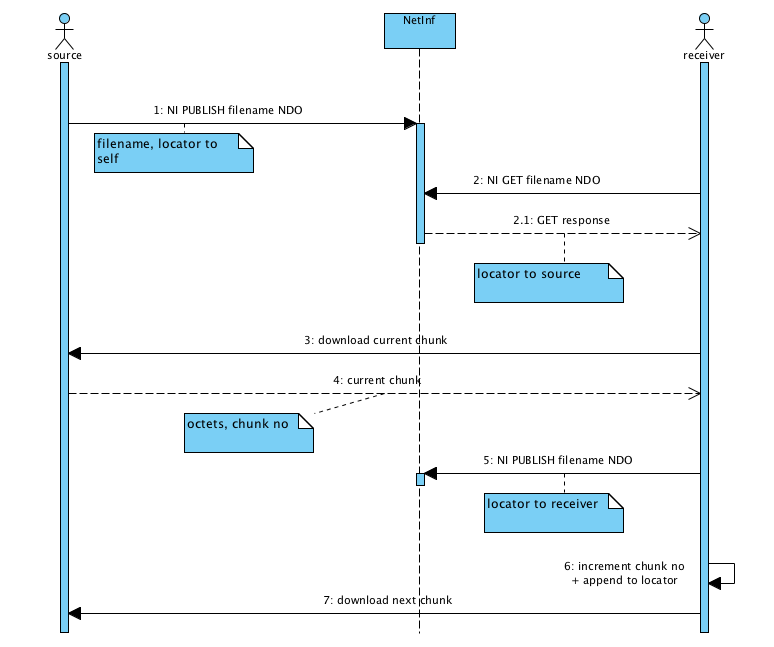
\includegraphics[scale=0.5]{./img/sequence_diagram_streaming.png}

\subsubsection{Testing criteria} 

For a simple test setup, in addition to our NetInf node, we need a receiving and a publishing client. A more sophisticated test could involve multiple receivers, to demonstrate the caching.

A use case we can use for testing is one where our source of the content is a pre-encoded video file of a particular size.

In the example below we will assume a video file of 700 megabytes.

A client (Publisher) will have a default chunk size which we will use to chunk up the source file. For example we will use 1 megabyte chunk size.

We can calculate from the Publisher that we will have 700 chunks, of 1 megabyte each numbered 0-699. 

A second client (receiver) knowing the name of the video file will then perform a GET request within the NetInf node (to keep things simple, we assume it knows the object's name already).

The client will now start generating consecutive GET's with the sequence numbers constantly increasing and expect to receive the appropriate chunk.

Also poll the NRS for new locators, to reduce the load of the network.

Until the GET's generate a 404 because the unique sequence number has increased past a chunk number that is not published.

\subsubsection{Extra notes}

Chunk size is going to be a configurable option in the publishing client.

The polling logic needs to be implemented in the client, that is how often the receiver should get a new chunk or check if a new chunk exists.  

\begin{thebibliography}{99}

\bibitem{otpInAction} Martin Logan, Eric Merritt, and Richard Carlsson. \textsl{Erlang and OTP in Action}. 2010.

\bibitem{ICNarticle} INFORMATION-CENTRIC NETWORKING Kostas Pentikousis et. al. IEEE Communications Magazine, July 2012

\bibitem{4ward} 4WARD project EU. 4WARD project home page. [Online]. http://www.4ward-project.eu/

\bibitem{masterthesis}
Hugo Negrette~Otaola and Miguel Sosa.
\newblock Using Multiple Transport Networks in NetInf Enabled Android Devices.
\newblock Master's thesis, KTH, School of Information and Communication
  Technology (ICT), 2012.

\bibitem{netinfproto}
D.~Kutscher, S.~Farrell, and E.~Davies.
\newblock The NetInf Protocol.
\newblock Internet-Draft draft-kutscher-icnrg-netinf-proto-00.txt, IETF
  Secretariat, Oct 2012.

\bibitem{opennetinf}
C.~Dannewitz, M.~Herlich, E.~Bauer, M.~Becker, F.~Beister, N.~Dertmann,
  R.~Hrestic, M.~Kionka, M.~Mohr, M.~M\"uhe, D.~Murali, F.~Steffen, S.~Stey,
  E.~Unruh, Q.~Wang, and S~Weber.
\newblock OpenNetInf Documentation Design and Implementation.
\newblock Technical Report TR-RI-11-314, University of Paderborn, Sept 2011.

\bibitem{plugin} Android Developers (n.d.). Installing the Eclipse Plugin. Android Developers. Retrieved January 8, 2013, from http://developer.android.com/sdk/installing/installing-adt.html

\bibitem{bundle} Android Developers (n.d.). Get the Android SDK. Android Developers. Retrieved January 8, 2013, from http://developer.android.com/sdk/index.html

\bibitem{hardware} Android Developers (n.d.). Using Hardware Devices. Android Developers. Retrieved January 8, 2013, from http://developer.android.com/tools/device.html\#setting-up


\end{thebibliography}

\end{document}
